
\documentclass[11pt,a4paper]{article}

\usepackage{tikz}
\usepackage{etex}
\newcommand*\mycirc[1]{%
  \begin{tikzpicture}[baseline=(C.base)]
    \node[draw,circle,inner sep=1pt](C) {#1};
  \end{tikzpicture}}
  \usepackage{rotating}
\usepackage{url}
% \usepackage[pdflatex]{graphicx}
\usepackage{amsmath,amssymb,fullpage,setspace,natbib,framed,multirow,rotating,ctable, comment}
\usepackage[colorlinks=true,anchorcolor=red,citecolor=blue,linkbordercolor={0 0 0},linkcolor=red,breaklinks=true,citebordercolor={0 0 0}]{hyperref}
\usepackage{adjustbox}
\usepackage[usenames,dvipsnames]{pstricks}
\usepackage{epsfig}
\usepackage{amsfonts}
\usepackage{tikz}
\usetikzlibrary{decorations.pathreplacing}
\usepackage{bm}
\usepackage{bbm}
\usepackage{ntheorem}
% \usepackage{amsthm}
\usepackage{subcaption}
\usepackage{appendix}
\usepackage{tabularx,cancel}

\DeclareMathOperator*{\argmin}{arg\,min}
\DeclareMathOperator*{\argmax}{arg\,max}


\newtheorem{theorem}{Theorem}[section]
\newtheorem{lemma}[theorem]{Lemma}
\newtheorem{proposition}[theorem]{Proposition}
\newtheorem{corollary}[theorem]{Corollary}
\newtheorem{assumption}[theorem]{Assumption}

\newenvironment{proof}[1][Proof]{\begin{trivlist}
\item[\hskip \labelsep {\bfseries #1}]}{\end{trivlist}}
\newenvironment{definition}[1][Definition]{\begin{trivlist}
\item[\hskip \labelsep {\bfseries #1}]}{\end{trivlist}}
\newenvironment{example}[1][Example]{\begin{trivlist}
\item[\hskip \labelsep {\bfseries #1}]}{\end{trivlist}}
\newenvironment{remark}[1][Remark]{\begin{trivlist}
\item[\hskip \labelsep {\bfseries #1}]}{\end{trivlist}}

\newcommand{\qed}{\nobreak \ifvmode \relax \else
      \ifdim\lastskip<1.5em \hskip-\lastskip
      \hskip1.5em plus0em minus0.5em \fi \nobreak
      \vrule height0.75em width0.5em depth0.25em\fi}

\newtheorem{hyp}{Hypothesis}
\makeatletter
\newcounter{subhyp}
\let\savedc@hyp\c@hyp
\newenvironment{subhyp}
 {%
  \setcounter{subhyp}{0}%
  \stepcounter{hyp}%
  \edef\saved@hyp{\thehyp}% Save the current value of hyp
  \let\c@hyp\c@subhyp     % Now hyp is subhyp
  \renewcommand{\thehyp}{\saved@hyp\alph{hyp}}%
 }
 {}
\newcommand{\normhyp}{%
  \let\c@hyp\savedc@hyp % revert to the old one
  \renewcommand\thehyp{\arabic{hyp}}%
}
\makeatother

% \usepackage{txfonts}
\newcommand{\eps}{\varepsilon}
\newcommand{\var}{\operatorname{var}}
\newcommand{\cov}{\operatorname{cov}}
\newcommand{\E}{\operatorname{E}}
\newcommand{\EE}{\mathcal{E}}
\newcommand{\qiffq}{\quad\iff\quad}
\newcommand{\revertstretch}{\setstretch{1.7}}

%\setlength{\textwidth}{6.5in}
%\setlength{\oddsidemargin}{-0.125in}
%\setlength{\evensidemargin}{-0.125in}
%\setlength{\topmargin}{0.1in}
%\setlength{\textheight}{8.25in} % was 9.25
%\setlength{\parskip}{\medskipamount}
%\setlength{\parindent}{15pt}

\revertstretch
\long\def\symbolfootnote[#1]#2{\begingroup%
\def\thefootnote{\fnsymbol{footnote}}\footnote[#1]{#2}\endgroup}

\colorlet{lightergray}{gray!15}  % this is used in one of the figures.

\renewcommand{\harvardurl}[1]{\textbf{URL:} \url{#1}}
% \newcommand{\datePath}{20160919}


%\newcommand{\pathToFigs}{./../analysis/output/value_approach/20170712} % 513} % 0919}
%\newcommand{\pathToTables}{./../analysis/output/value_approach/20170712} %513} % 0405} % 919}
%\newcommand{\defaultS}{85}
%\newcommand{\defaultSpan}{0_75}

%======================================================

\begin{document}
\vspace*{1.5in}
\begin{center}
% ======================================================
{\huge
{Comparing strategic voting incentives in \\ plurality and instant-runoff elections}\footnote{This version: \today. %I thank \ldots .
}}\\[0.3cm]%  Some ideas in this paper appeared in an earlier draft coWe thank seminar audiences at Barcelona IPEG, IAST Toulouse, the University of Toronto, and the University of Lancaster.
% }}\\[0.3cm]

% ======================================================
\Large \textbf{Andrew C. Eggers}\symbolfootnote[2]{Nuffield College and Department of Politics and International Relations, University of Oxford, UK. email: \texttt{andrew.eggers@nuffield.ox.ac.uk}}\\[0pt]
\textbf{Tobias Nowacki}\symbolfootnote[2]{Stanford University. email: \texttt{tnowacki@stanford.edu}}\\[0pt]

% PRELIMINARY AND INCOMPLETE
%======================================================
\end{center}
\bigskip
\bigskip
\bigskip
\bigskip

\begin{center}
\textbf{Abstract}
\end{center}
\begin{quotation}\singlespacing
\noindent % Well-known theorems show that there is no strategy-proof voting system, but 
Reformers and researchers often speculate that some voting systems induce less strategic voting than others, but existing research is unhelpful in assessing these conjectures because it is overwhelmingly based on the unrealistic assumption that voters know exactly how others will vote. We propose a general approach to assessing strategic voting incentives given realistic uncertainty about election outcomes. We use this approach to compare strategic voting incentives in three-candidate plurality and instant-runoff (IRV) elections, drawing on preference data from 160 electoral surveys. We show that the common conjecture that strategic voting incentives are smaller in IRV than in plurality is correct: for the full range of beliefs about how strategic one thinks other voters will be, the expected benefit of being a strategic voter rather than a sincere voter is smaller in IRV than in plurality. % , and the differential is larger when one expects other voters to be more strategic. 
%Our baseline approach measures whether and by how much a voter would benefit from an insincere vote   
%previous theoretical and empirical work provides little guidance about how systems differ in the extent to which 
% all voting systems are in principle vulnerable to strategic voting,   
%The instant-runoff voting system (IRV, also known as AV, RCV, preferential voting, and single-winner STV) is used to elect legislators throughout Australia, mayors in London, San Francisco, and several other major cities, and (recently) members of Congress from the U.S. state of Maine. Advocates argue that IRV reduces voters' incentive to vote strategically compared to plurality, but that claim has never been rigorously assessed. Using new methods for calculating the probability of pivotal events in IRV elections and preference data from 160 election surveys, 
% In the alternative vote system (AV, also known as preferential voting in Australia and IRV or RCV in the United States), voters rank candidates and a majority winner is chosen through a successive elimination process. We address some key questions about strategic voting in AV. %  What types of strategic voting (if any) should we expect? Which candidates benefit? Based on a decision-theoretic analysis of three-candidate AV elections, we show that (1) insincere forms of manipulation (e.g.\ vote for $C$ to elect $A$) are unlikely given reasonable uncertainty about election outcomes, and (2) centrist candidates tend to benefit from strategic voting. 
\end{quotation}
\revertstretch


\newpage


\section{Introduction} % Measuring and comparing strategic voting incentives across voting systems} 

%People make comparisons of strategic voting incentives in policy discourse. \ldots 
%
%Some academic research comparing strategic voting incentives. \ldots 
%
%But what's the problem with these approaches? \ldots 
%
%
%\subsection*{Our approach, v2} 
%
%\subsubsection*{The basic problem}

Social choice theory tells us that no reasonable voting system is completely immune from strategic voting (cites). %: if a voting system is responsive to voters' sincere preferences (as it should be) and is unable to tell the difference between ballots that reflect sincere and insincere preferences (as it must be), then whenever there are three or more candidates there is inevitably some circumstance in which a voter would benefit from submitting a ballot that does not reflect her true preference.\footnote{The Gibbard-Satterthwaite theorem shows this for ordinal voting systems, i.e.\ systems that use candidate rankings as inputs. XXX extends this to other results, e.g.\ approval voting. TODO: cite.} 
It is reasonable to suspect, however, that %while no systems are immune from strategic voting 
some systems are likely to be more susceptible to strategic voting than others. 
% Because susceptibility to strategic voting is typically viewed as a shortcoming of electoral systems \citep[though see][]{dowding2008praise}, debates about electoral system reform commonly include claims that one system is more susceptible than another. 
For example, in advance of the 2011 UK referendum to replace plurality parliamentary elections with a form of instant-runoff voting (known as the alternative vote in the UK), Deputy Prime Minister Nick Clegg claimed that IRV ``stops people from voting tactically and second-guessing how everybody else will vote in their area'';\footnote{``The Coalition
Government’s programme of political and constitutional reform: Oral and written evidence'', 15 July 2010, HC 358-i, published 22 October 2010 (\href{https://publications.parliament.uk/pa/cm201011/cmselect/cmpolcon/358/358i.pdf}{link}). By ``tactical voting'' Clegg likely means submitting a ballot that differs from one's sincere preference.} \emph{other non-academic claims here}. Prominent scholars have made similar conjectures. % scholars who have compared strategic voting incentives in IRV and plurality, 
\citet[][95]{cox1997making}, for example, notes that more information is needed to vote strategically in IRV than in plurality, as does \citet[][pp.\ 6-7]{renwick2011alternative}, who concludes that IRV would ``reduce but not eliminate incentives for tactical voting'' compared to plurality, while \citet[][p.\ 228]{dummett1984voting} maintains that ``a voter who has understood the workings of the procedure, and who has some information about the probable intentions of the others, will have nearly as much incentive to vote strategically'' in IRV as in plurality elections.

Considering that the question of which system is more susceptible to strategic voting seems to be relevant to many policymakers and academic researchers alike, previous research provides a surprisingly unsatisfying answer.  As noted above, the classic theorems show that all reasonable systems could produce a \emph{manipulable} voting result, i.e.\ a configuration of ballots such that one or more voters would be better off submitting an insincere ballot than a sincere one. Building on these theorems, a large literature (mostly in mathematics and computer science) has assessed the likelihood of such a manipulable result for different voting rules given some assumption about the distribution of possible voting outcomes \citep[e.g.][]{chamberlin1985investigation,nitzan1985vulnerability,saari1990susceptibility,favardin2006some}.\footnote{A closely related set of papers assesses the probability of results that violate monotonicity and other desirable properties of choice rules \citep{plassmann2014frequently,ornstein2014frequency,miller2017closeness}.} %TODO: more recent manipulability studies 
But these studies are of little use for assessing susceptibility to strategic voting, even if we accept their assumptions about likely voting outcomes, because they do not take into account uncertainty about others' votes: they essentially ask how likely a voter is to \emph{regret} a sincere vote after the election takes place, not how likely a voter is to \emph{foresee} that an insincere vote would be optimal before the election takes place. A system can only be susceptible to strategic voting if voters could anticipate, given reasonable beliefs about the relative likelihood of different election outcomes, that an insincere vote would be better than a sincere one. Previous research on voting systems' susceptibility to \emph{ex post} manipulation thus has little to say about their susceptibility to \emph{ex ante} strategic voting. %Put differently, manipulability is a necessary but not sufficient condition for susceptibility to strategic voting. 
% there are circumstances where the voter could do better by not voting sincerely (i.e.\ the system is manipulable) \emph{and} the voter's beliefs about the relative likelihood of these circumstances point indicate that a particular insincere vote would be better than a sincere one. 

To see the difference uncertainty makes, % how the \emph{ex ante} perspective and the \emph{ex post} perspective can yield diametrically different conclusions, 
%  a system that is highly manipulable when we assume voters are certain about others' voters but may not be susceptible to strategic voting when we assume voters have realistic information, 
consider a three-candidate plurality election in which the three candidates are expected to have roughly equal support. To evaluate manipulability using the typical \emph{ex post} approach, we would first draw a large number of simulated elections from a distribution capturing our beliefs about likely outcomes; we would then count the proportion of cases in which an insincere vote could yield a better outcome for some voter. Given the assumption that the three candidates have roughly equal support, we would expect a roughly equal number of ties for first between each pair of candidates, each of which provides an opportunity for a voter whose first choice finishes third to obtain a better outcome by voting for their second choice; the more such ties, the more manipulable the system would appear to be. But when we consider the problem from the \emph{ex ante} perspective, we arrive at a very different conclusion. If a tie for first is equally likely between each pair of candidates, a sincere vote is always optimal; fundamentally, this is because ties that reward sincerity are more numerous and have higher stakes on average than ties that reward insincerity.\footnote{A sufficient condition for a sincere vote to be optimal in a three-candidate plurality election is that, given preference ordering $abc$, a $bc$ tie and an $ac$ tie are equally likely.} The possibility of manipulable results means little for strategic voting unless, given reasonable uncertainty, a voter could discern that a result that would reward an insincere vote is substantially more likely than a result that would reward a sincere vote. 

In this paper, we propose a general approach to assessing strategic voting incentives in the presence of uncertainty and use it to %comparing strategic voting incentives 
assess whether plurality or instant-runoff elections are more susceptible to strategic voting (the question on which Clegg, Cox, and Dummett all offered views above). 
Our measure of strategic voting incentives in a given electoral system is the answer to the question, ``How much should a consequentialist voter (i.e.\ one who cares only about election outcomes) be willing to pay to vote strategically rather than sincerely?'' %``How much would the average citizen benefit from being a strategic voter (i.e.\ one who chooses the optimal ballot given her preferences and informed but imprecise beliefs about others' votes) rather than a sincere voter (i.e.\ one who simply chooses the ballot that most closely reflects her preferences)?'' Put differently, how much should the average voter be willing to pay to be strategic rather than sincere? 
The answer to this question depends on what we assume about voters' \emph{preferences} and \emph{beliefs}. For preferences, we use election surveys in the Comparative Study of Electoral Systems (CSES) in which voters are asked to rate each party on a 0-10 scale; this yields over 230,000 sets of preferences in 160 different elections.\footnote{In each survey we use preferences over the top three parties (in terms of national vote share) only.} Next, we model voters' beliefs about possible election outcomes as a probability distribution satisfying two criteria: first, the precision of the distribution is consistent with the empirical predictability of election outcomes; second, the location of the distribution is consistent the preference data (i.e.\ what other voters in the same election want) and one of a range of assumptions about the prevalence of strategic voting. This approach allows us to measure, for each voter and a given assumption about how strategic \emph{other} voters are expected to be, the expected benefit of strategic voting compared to sincere voting and, ultimately, to compare this benefit across different voting systems. 

We find that, consistent with some of the conjectures noted above, the incentive to vote strategically is considerably lower in IRV than in plurality elections. Decomposing the expected benefit of voting strategically, we observe that IRV is more resistant to strategic voting both because the probability of benefiting from a strategic vote is lower and because the magnitude of that benefit (when it exists) is smaller. We find that the expected benefit from strategic voting is lower in IRV regardless of how strategic other voters are expected to be, but the gap between plurality and IRV is larger the more strategic other voters are expected to be: as other voters become more strategic, the probability of benefiting from a strategic vote increases in plurality  (because strategically deserting a \emph{trailing} candidate becomes more attractive when other voters are expected to do so) but decreases in IRV (because strategically deserting a \emph{leading} candidate becomes  less attractive when other voters are expected to do so). 

%  the more strategic one expects other voters to be, the more likely one is to benefit from being strategic in plurality, while the reverse is true in IRV. (Fundamentally, this is because deserting a trailing candidate in plurality becomes more attractive when other voters are expected to do so, while deserting a leading candidate in IRV becomes less attractive when other voters are expected to do so.)   

\begin{comment} 
We assume that each voter knows the approximate proportion of all voters with each sincere ordering of the candidates (e.g.\ the proportion who rate $A$ above $B$ and $B$ above $C$). We then consider a sequence of beliefs that a voter could reasonably hold about how strategic other voters might be, ranging from the belief that all other voters will vote sincerely to the belief that all voters will vote according to a strategic voting equilibrium. (This sequence can be thought of    
% We assume that each voter knows the rough proportion of all voters with each sincere ordering of the candidates (e.g.\ the proportion who rate $A$ above $B$ and $B$ above $C$) and they expect the election outcome to approximate these proportions.\footnote{More specifically, we assume they have Dirichlet beliefs centered on the proportions observed in the survey; we examine results for various assumptions about belief precision.} 
Finally, for each voter we compare the expected utility if the voter is strategic (i.e.\ chooses the optimal ballot given her beliefs about others' votes) and if the voter is sincere (i.e.\ chooses the ballot that most closely reflects her sincere preference); the difference between these two   

each voter's strategic voting incentives at each belief in this sequence. %  given these beliefs about likely outcomes and the voting system. % (ii) the voter's ratings of the parties (which we use as proxies for the voter's cardinal utility), and (iii) the voting system. 
% Put differently, in our baseline approach we measure the strategic voting incentives of voters in an election survey under the assumption that the voters observe summary statistics from the survey and are level-1 strategic voters (i.e.\ those who are strategic but think that others are not). Because it may be unrealistic to assume that strategic voters expect no one else to be strategic, we also extend the baseline approach to examine the strategic voting incentives for level-2 strategic voters (i.e.\ those who believe that some others are level-1 strategic voters); comparing the incentives of level-1 and level-2 strategic voters sheds light on the way strategic voting behavior is interdependent in a given system.   

We apply this approach to comparing strategic voting incentives in plurality and instant-runoff elections. Plurality is the most-studied and most-used single-winner election method in the world. Instant-runoff voting (IRV, also known as the alternative vote, preferential voting, ranked-choice voting, and single-winner STV\footnote{We choose to call it instant-runoff voting because that term describes the rule most accurately.}) is less well known and far less studied. %TODO: cites 
In an instant-runoff election, voters rank candidates and candidates are successively eliminated until only one remains. IRV is used in Australia to elect members of the lower house for the federal government and all state governments; it is used to elect mayors in Sydney, London,  San Francisco, and ten other American cities;\footnote{Minneapolis, MN; Portland, ME; Takoma Park, MD; Berkeley, CA; Oakland, CA; San Leandro, CA; Basalt, CO; Telluride, CO; St.\ Paul, MN; Santa Fe, NM.} it is used to elect the head of state in Sri Lanka (where the position holds real power) as well as in India and Ireland (where the position is essentially ceremonial). IRV  has become a common reform proposal in the U.S., and in 2018 the system was used for the first time to elect a member of the U.S.\ Congress. Like Nick Clegg above, reformers favoring IRV commonly argue that the system reduces the incentive to vote strategically compared to plurality. Part of our purpose is to evaluate this claim rigorously. We also seek to determine how strategic voting affects the relative performance of the two systems: for example, IRV is at least as likely as plurality to elect the Condorcet winner given sincere voting, but does this advantage persist when voters are strategic?   

\end{comment}

% Table \ref{tab:examples} provides some examples of RCV elections. As a system for national legislative elections, RCV is used only in Australia and Papua New Guinea, though RCV is used in the US state of Maine to elect members of both house of Congress beginning in 2018. It is used to elect the head of state in Sri Lanka (where the position holds real power) as well as in India and Ireland (where the position is essentially ceremonial). RCV is used to elect the lower house in all Australian states. It is used to elect the mayor of London, the mayor of Sydney and several other Australian cities, and the mayor and city council of San Francisco and ten other U.S.\ cities.\footnote{Minneapolis, MN; Portland, ME; Takoma Park, MD; Berkeley, CA; Oakland, CA; San Leandro, CA; Basalt, CO; Telluride, CO; St.\ Paul, MN; Santa Fe, NM} 
%Whether judging by number of seats filled or number of ballots cast, RCV appears to be the third most common single-winner system of election: the use of plurality elections in India alone swamps the use of RCV globally, as does the use of majority runoff elections in France alone, but no other single-winner system (such as Borda Count,  approval voting, or Condorcet methods) is used anywhere nearly as widely as RCV.\footnote{The only single-winner elections for public office that we know of that use a system other than plurality, majority runoff, or RCV occur in Vanuatu, where an electorate of around 8,000 uses Borda Count to elect 19 legislators.}    


% We find \ldots

% Looking at strategic voting incentives in these two systems is particularly relevant because if voters are sincere IRV is weakly better at electing the Condorcet winner, but it is unclear whether IRV retains this advantage when voters are strategic. \emph{Continue.}  

We emphasize that our focus in this paper %  does not address whether voters actually 
% on this paper 
 is on the \emph{incentive} to vote strategically given reasonable uncertainty about others' votes, not the empirical prevalence or practicability of strategic voting. In order to detect the strategic incentives we measure in this paper, a voter needs basic information about the likely prevalence of each ballot type, a good understanding of the voting system, and the ability to reason strategically. Many voters may lack one or more of these ingredients \--- especially in IRV, which previous researchers have noted is more complicated to manipulate than plurality and other voting systems.\footnote{In a framework where voters are certain about each others' votes, \citet{bartholdi1989computational} use computational complexity theory to assess the difficulty of manipulating an outcome in various voting systems; \citet{bartholdi1991single} argues that manipulation in IRV is uniquely complex. \citet{cox1997making} and \citet{renwick2011alternative} also note that strategies in IRV are more logically complicated than strategies in plurality, which suggests that some voters may find it too difficult to even attempt.} In this sense, our paper sheds light on strategic voting incentives as these incentives might be computed by a voting advice service or perceived by a highly sophisticated party strategist who has well-formed (though imprecise) beliefs about election outcomes and can work through the implications of alternative voting strategies in a given system. % possible  understands exactly how the system works, and can combine her beliefs and understanding of the system to determine what to do. % (Thus this is the incentive as it might be computed by a voting advice service.) 
Future research can assess whether actual voters can perceive and act on these incentives, but this paper provides insight on whether these incentives exist, how strong they are, in what direction they point, and how they are likely to affect outcomes.
 
  
%  in these two systems given realistic levels of uncertainty; we do not assess whether voters actually could or would vote strategically.  
%A third alternative would characterize susceptibility to strategic voting by measuring the cognitive difficulty of identifying the optimal vote. For example, in the context where voters are certain about each others' votes, \citet{bartholdi1989computational} use computational complexity theory to assess the difficulty of manipulating an outcome in various voting systems. More prosaically, \citet{cox1997making} and \citet{renwick2011alternative} note that strategies in IRV are more logically complicated than strategies in plurality, which suggests that some voters may find it too difficult to even attempt. Our paper ignores the computational challenge of identifying the correct strategic vote. It assesses strategic voting incentives as they would be perceived a voter who has realistically imprecise beliefs about likely election outcomes but no difficulty in determining, based on that information and her preferences, the optimal vote.       



  

% These ratings provide the basis for our assumptions about both preferences and beliefs: we use the ratings as proxies for utility scores, essentially assuming that a purely strategic voter would choose the ballot that maximizes the expected rating of the winner; and we assume that voters know the proportion of other voters with each sincere preference ordering and expect everyone else to vote sincerely. Put differently, we study the optimal voting behavior of respondents to election surveys under the assumption that those respondents also see the survey (or at least summary statistics from it) and are level-1 strategic thinkers (i.e.\ they vote strategically but believe others do not).   


   
 

 

% noting that a voter would need more information in IRV than in plurality to know when a sincere vote is not the best option.\footnote{Alan Renwick, ``The Alternative Vote: A Briefing Paper'', \emph{Political Studies Association} 24 March 2011, pp.\ 6-7. Renwick also notes that IRV and plurality rewarded a tactical vote in different circumstances.}      


%This apparently theoretical question quickly becomes largely empirical. The social choice theorems tell us that, for any reasonable system, we can identify a combination of voter preferences and beliefs about likely outcomes such that the voter optimally votes insincerely; but in the same system we can also specify a combination of voter preferences and beliefs about likely outcomes such that the voter optimally votes sincerely, and it is not obvious how to weigh the two possibilities.\footnote{In plurality, for example, a voter with preference ordering $abc$ (i.e.\ who  prefers candidate $a$ to candidate $b$ to candidate $c$) optimally votes for $b$ if she expects only $b$ and $c$ to have a chance of tying for first, while she optimally votes for $a$ if she expects only $a$ and $b$ to have a chance of tying for first.} To characterize the susceptibility of any voting rule to strategic voting, we therefore need to make assumptions about the likelihood of different possible outcomes, the distribution of preferences in the electorate, and how beliefs and preferences relate. There is no single theory that tells us what beliefs and preferences to assume. In a plurality election, for example, we could assume that voters expect only two candidates to receive all support (as predicted by almost all equilibrium models), but most models do not specify \emph{which} two candidates should receive support, nor does any model tell us where the underlying distribution of preferences comes from. Theory is even less helpful in systems other than plurality because there has been far less theoretical work (TODO: cite bouton etc).   


\begin{comment} 
Pattanaik 1975 
  
Chamberlin 1985 -- monte carlo; IC and 4D spatial; ex post. finds Hare method less manipulable 
Nitzan 1985 -- same thing. 
Saari 1990 -- analytical approach similar to above
Favardin Levelley: good lit review, questioning IC, using different quasi-eqm ideas, using IAC.  
Walsh 2010: "empirical" investigation of manipulability of STV. but: ex post; pref data not actually empirical.
Baharad Neeman 2002  not equiprobability but probably ex post? 
Lepelley and Valognes 2003   not equiprobability but probably ex post? 
Nurmi's book?  in SSL at  JF1001.NUR

So we have a set of papers looking at probability of paradoxes using more realistic distributions of results 
-- Allard 1996 looking at IRV in the UK. In "voting matters" -- can't find it. 
-- Plassman and Tideman: good for empirical realism in voting situations.
-- Ornstein and Norman has a bit of competition among the candidates, starting from random positions 
-- Miller: probability of monotonicity failure in simulated IRV elections; random, single-peaked, clone candidate (divided majority), English preference pattern.  
To take away: some empirical efforts; some spatial; a little bit towards eqm but not much. 
\end{comment} 




\begin{comment} 

\emph{Characterize confusion/disagreement/vagueness that we can resolve. Some naive statements, typically vague, about how AV addresses the problem of tactical voting \--- either demonstrably false or vague. In response, statements that say no it is bad, somehow even worse, etc. Properties, non-monotonicity. Dummett, Brams and Potthoff maybe. Qualifications/defenses vague about incentives being lower etc. And pointing to the Australian case, where strategic voting does not seem to be much of a consideration.} 


A consideration of strategic voting is also important for assessing the performance of RCV. It is well known that the first-preference winner usually wins RCV elections in Australia \citep[e.g.][p.~83]{farrell2006australian}. Several commentators have concluded from this observation that RCV and plurality is likely to produce the same outcome, %Who? Butler, Rydon, Rae making comments about similarity on page 82, but not sure if this is what they mean -- I have notes on this somewhere 
but this conclusion depends on the assumption that strategic voting behavior would be similar in the two systems, i.e.\ that the first-preference winner would be same.  

\citet[][p.~82-83]{farrell2006australian} note that over the 1949-2001 period an increasing proportion of Australian House races have required elimination rounds before the winner was decided (or, put differently, fewer races have seen one candidate win a majority of first-preference votes). They attribute this in part to an increase in strategic voting, though they give no explanation for this judgment and, as we will show below, strategic voting could in fact either increase or decrease support for leading candidates.\footnote{\citet{farrell2006australian} seem to argue that strategic voting should be thought of fundamentally differently in preferential systems because ``the range of choices available to voters is greater'' (pg.\ 127). Still, they ultimately embrace a definition of strategic voting that is essentially the same as ours: strategic voting means placing ``a higher priority on electoral outcome than on preferred candidate'' or %  state that, ``When assessing strategic voting under preferential systems, therefore, the issue is less one of a voter 
``trying to influence the election outcome by voting \ldots %non-sincerely, and more one of trying to do so by deploying her vote 
in as efficient a manner as possible'' (127). Their key point seems to be that because ballots in preferential systems require voters to rank candidates, a ballot could be sincere in some rankings and insincere in others, which requires thinking of insincere ballots somewhat differently from in plurality elections, and that (pg.\ 173) strategic voting in preferential systems needs more attention.} % a strategic voter who supports the leading candidate may try to affect the order of elimination by moving a less-preferred candidate above her favorite, which could lead to fewer candidates winning with a majority of first-preference votes, but it may also lead to     
\citet[][p.~129]{farrell2006australian} also assert that how-to-vote cards distributed by the parties are designed ``to ensure the election of the party's candidate and maximum damage to the party seen as the greatest threat.'' But on reflection it is not clear that the existence of how-to-vote cards is itself evidence of strategic behavior. In a three-candidate race, the only way to be sure that a party is directing voter strategy would be if a party's how-to-vote card listed \emph{another party's candidate} first on the card, which has apparently never happened. This follows from the theorem and Dummett's observation that if one's true preference is $ABC$ one should consider only ballots $ABC$, $BAC$, and $CAB$. To put the point another another way, suppose that $A$ and $B$ were likely contenders for the seat and $C$ is expected to be a minor candidate. Some of the literature (and that range voting guy) seems to suggest that for a voter with sincere preference $ABC$ it might make sense to put $B$ last, i.e.\ vote $ACB$, but in fact it cannot (at least in the pivotal voter model): if $A$ is eliminated, giving preferences to $C$ may indeed help to defeat $B$, but only by electing $C$, which is purportedly the voter's last choice. If there is indeed a reason for a contending party $A$ to list its main opponent $B$ last on an HTV card (when the party and its supporters actually prefer $B$ over some other party $C$), the logic seems to be completely different. Perhaps in doing so $A$ hopes to convince voters who sincerely prefer $C$ that $A$ is sympathetic to their concerns (or that $A$ is at least as sympathetic to their concerns as $B$ is). This strategy could only make sense, however, if the set of $C$ supporters who are susceptible so such ploys is large relative to the set of voters who are indifferent between $A$ and $B$ and might be dissuaded from voting for $A$ by this maneuver.   We should get this book again when we look at the history and prevalence -- details about use in state elections here. 


We focus on two broad questions about strategic voting in RCV elections. First, we ask about the voter's incentive to vote strategically: what rewards might a voter expect from voting strategically in an RCV election? We consider the problem of a voter who has well-formed (but imprecise) beliefs about other voters' votes and has no trouble determining her own optimal vote given those beliefs. How likely is it that such a voter would benefit from a non-sincere vote, and by how much? How concerned should the voter be about the voting paradoxes that are known to afflict RCV and other runoff systems (the no-show paradox and non-monotonicity)? To what extent does the optimal vote of such a voter depend on the voter's beliefs about how strategic \emph{other voters} are? Second, we ask about how the performance of RCV depends on voters' strategic behavior. If voters vote sincerely, RCV is weakly more likely than plurality to elect the Condorcet Winner in a three-candidate case.\footnote{To see this, note that neither system elects the Condorcet winner if that candidate finishes last in first preferences (i.e.\ is least often ranked first) and both systems elect the Condorcet winner if that candidate finishes first in first preferences, while RCV (but not plurality) elects the Condorcet winner if that candidate finishes second in first preferences. With more than three candidates, it is possible for plurality to elect the Condorcet winner while RCV does not. (Suppose four candidates, with the Condorcet winner receiving the largest number of first-place votes. This candidate would be elected in plurality but could be eliminated in RCV if, after the fourth-placed candidate is eliminated and her votes redistributed, the second- and third-placed candidates move ahead of the leader.)} But does this advantage of RCV over plurality hold when voters vote strategically? (\emph{Are there other ways to assess performance?}) 

In this paper, we address some of the shortcomings in prior literature by studying the voter's decision problem in an RCV election. Following essentially all of the formal literature on voting systems, we focus on the three-candidate case; this keeps the complexity manageable while highlighting all of the important features, and has the added benefit that with just three candidates many variants of RCV operate identically (as discussed further below). We begin by modeling the beliefs a voter might have about election outcomes (in terms of the frequency of each type of permitted ballot) and calculating the probability of a marginal ballot being decisive in each possible way as a function of these beliefs. 
Applying this approach to recent RCV elections for which detailed ballot frequency data is available, we provide new estimates of the empirical relevance of the no-show paradox and non-monotonicity paradox.   
We then assess how precise a voter's beliefs would need to be for a non-sincere vote to become advantageous: if the voter is completely agnostic about likely election outcomes a sincere ballot is always optimal, but how much information is necessary before it could become clear that a non-sincere ballot is optimal? It turns out that (given the voter understands the system) a non-sincere vote can emerge as optimal even with quite vague beliefs about likely ballot frequencies. This tends to support \citet{dummett1984voting} and others who postulated that strategic voting in RCV elections may not require unreasonable amounts of information. 

Next, we highlight two features of strategic voting in RCV as compared to plurality elections that may help explain why, despite the apparent feasibility of strategic voting in either system with imprecise beliefs about election outcomes, strategic voting seems to be unimportant in RCV elections in Australia and elsewhere. First, we show that the magnitude of the benefit of an insincere vote (compared to a sincere vote) tends to be small in RCV compared to in plurality. This implies that, if sincere voting has a small expressive benefit (or insincere voting a small cognitive cost), this benefit/cost may completely swamp the strategic advantages of an insincere vote in RCV but not in plurality.  Second, we show that given a poll of voting intentions, the optimal vote in RCV depends on one's beliefs about whether \emph{other voters} are strategic much more than is the case in plurality elections.\footnote{More specifically (as we detail below), if one believes that a proportion $\lambda$ of other voters are level-1 strategic thinkers, i.e.\ they are strategic but they think no one else is, then one's optimal vote rarely depends on $\lambda$ in plurality elections but often depends on $\lambda$ in RCV elections.} This strategic interdependence may simply reduce voters' certainty about likely election outcomes in RCV (and may do so even beyond the low threshold where an insincere vote emerges as optimal), but it may also complicate the voting problem for voters who (as \citet[][p.\ 213]{dummett1984voting} suggests most do) think of the optimal vote as the answer to the question, ``What should all voters with my preferences do?'' These two factors may (along with the obvious complexity of the strategic problem in RCV elections) explain why strategic voting is empirically rare despite being theoretically possible in RCV elections. 

Finally, we undertake an exercise to assess the likely impact of strategic voting on outcomes in RCV elections: if, despite the complexity, the muted incentives, and the strategic interdependence of strategic voting in RCV elections, a subset of voters responded strategically (but myopically, and in a level-1 manner) to a poll, how would the expected result compare to the expected result under sincere voting? In a simulation using preference data from 162 elections in 56 countries from the Comparative Study of Electoral Systems (CSES), we show that a moderate amount of (myopic, level-1) strategic voting in RCV makes the Condorcet winner slightly more likely to win. The reason seems to be that, when preferences are fairly single-peaked, the centrist candidate (i.e.\ the one who tends to be the second choice of other candidates' supporters), who is likely to be the Condorcet winner, tends to attract the support of strategic voters. %this is also true in plurality
Thus in contrast to \citet[][p.\ 227-228]{dummett1984voting}, who speculated only that RCV with strategic voting was unlikely to yield much worse outcomes than RCV with sincere voting, we show that, at least by the Condorcet criterion and in the conditions of our simulation, the performance of RCV actually improves as voters becomes more strategic. The relationship is non-monotonic, however: as the proportion of myopic, level-1 strategic voters (i.e.\ those who respond strategically to a poll as if no one else would do so) goes above about $1/5$, RCV's performance starts to deteriorate, as (for example) a Condorcet winner whose victory is almost assured under sincere voting loses too much support from strategic voters who try to affect the order of elimination. Still, RCV performs better than plurality by the Condorcet criterion as long as the proportion of myopic strategic voters is below about $1/2$. 


% would only venture that RCV ``will probably not fail [to produce the fairest outcome] more frequently when strategic voting occurs'', we show that a moderate amount of (myopic, level-1) strategic voting tends to make the Condorcet winner win more frequently \emph{(in fairly single-peaked situations?)}. This is because, in a situation where preferences are mostly single-peaked (in the sense that one ``centrist'' candidate is unlikely to be someone's least favorite candidate), the Condorcet winner tends to drain away another candidate's support while the Condorcet winner's own supporters optimally vote sincerely.  

%% Can I set this up? 
%% I can adapt the iterative thing I did.         

% Things I need to write: 
	%% some motivation stuff: Dummett quotes, what we know and don't know. 
	%% some stuff about where AV is used, which cases this paper speaks to
	%% a gentle introduction to tactical voting incentives in AV, perhaps by analogy to two-round 


\subsection{RCV and its use in elections around the world} 

The fundamental characteristics of elections that we study in this paper are (1) voters rank candidates, and (2) the winner is chosen by an elimination procedure that favors candidates with more first-place votes. A variety of terms are used to describe such elections, including ``alternative vote'', ``preferential voting'', ``instant-runoff voting'', ``ranked-choice voting'', ``supplementary vote'', and ``contingent vote''; the last two are usually used to describe a variant (which we describe below), but the first four terms are used to describe the same basic process in different countries.\footnote{``Ranked-choice voting'' and ``instant-runoff voting'' are popular in the US, ``preferential voting'' in Australia, and ``alternative vote'' in the UK.} %and may reflect the marketing efforts of advocates. 
Unfortunately, none of the terms says much about the procedure they describe. ``Ranked-choice voting'', for example, would seem to describe any system in which voters submit ordered lists of preferences (including the Borda Count and any Condorcet  method), ``preferential voting'' would seem to refer to any of these systems plus others in which preferences are submitted in some other format such as scores or ratings, and ``alternative vote'' makes us ask ``alternative to what?''\footnote{The most descriptive might be ``single-winner STV'', which is used in Ireland to describe presidential elections.} For want of a better term, and because of recent interest among American reformers who use the term ``ranked-choice voting'', we will use the term ``RCV'' to describe the system we study in this paper.  

Table \ref{tab:examples} provides some examples of RCV elections. As a system for national legislative elections, RCV is used only in Australia and Papua New Guinea, though RCV is used in the US state of Maine to elect members of both house of Congress beginning in 2018. It is used to elect the head of state in Sri Lanka (where the position holds real power) as well as in India and Ireland (where the position is essentially ceremonial). RCV is used to elect the lower house in all Australian states. It is used to elect the mayor of London, the mayor of Sydney and several other Australian cities, and the mayor and city council of San Francisco and ten other U.S.\ cities.\footnote{Minneapolis, MN; Portland, ME; Takoma Park, MD; Berkeley, CA; Oakland, CA; San Leandro, CA; Basalt, CO; Telluride, CO; St.\ Paul, MN; Santa Fe, NM} 
Whether judging by number of seats filled or number of ballots cast, RCV appears to be the third most common single-winner system of election: the use of plurality elections in India alone swamps the use of RCV globally, as does the use of majority runoff elections in France alone, but no other single-winner system (such as Borda Count,  approval voting, or Condorcet methods) is used anywhere nearly as widely as RCV.\footnote{The only single-winner elections for public office that we know of that use a system other than plurality, majority runoff, or RCV occur in Vanuatu, where an electorate of around 8,000 uses Borda Count to elect 19 legislators.}    

\begin{table} \caption{Examples of RCV elections around the world (\emph{replace this with something comprehensive?})  \label{tab:examples}} 
\begin{tabular}{p{4cm} p{3cm} p{3cm} p{2cm} p{3cm}}
\textbf{Setting}& \textbf{Office(s)} & \textbf{Ballots cast in recent election} & \textbf{Rankings allowed} & \textbf{Elimination procedure} \\   \hline
Australia & Federal representative &  13.5M (2016) & Full  only & Successive \\[0.5cm] 
% W.\ Australia, S.\ Australia, Tasmania & State legislative assembly   & 1.4M (2018), 1M (2018), 334k (2018) & Full rankings required & Successive \\  
Queensland, Victoria, and New South Wales & State representative  & 11M (2015-2017) & Any  & Successive\\[0.5cm] % %2.8M (2017), 3.5M (2014), 4.5M (2015), 100k (2016) 
Sri Lanka & President  & 12M (2015) & Up to 3 & All but top 2 \\[0.5cm]
London, UK & Mayor & 2.6M (2016) & Up to 2 & All but top 2  
\end{tabular} 
\end{table}

There are two important differences within the RCV family of elections. The first difference relates to how candidates are eliminated. In most RCV-like elections, candidates are eliminated one by one: when all the ballots have been tallied, the candidate with the fewest first-place votes is determined and eliminated from all ballots, after which the candidate with the fewest first-place ballots is again determined and eliminated, and so on until one candidate attains a majority. In some elections (often referred to as ``supplementary vote'' or ``contingent vote''), all but the top two candidates are eliminated in a single step; examples include elections of the Sri Lankan president and London mayor.\footnote{These elections closely resemble a top-two runoff election held using one set of ballots. Unfortunately, the term ``instant-runoff election'' usually refers to an election using the standard successive elimination procedure.} The other difference relates to the kinds of ballots voters may submit. In federal elections and some state elections in Australia, voters must rank every candidate or the ballot is invalid. In other state elections in Australia, elections of the Irish president, and elections of mayor and city council in St.\ Paul, MN, and Santa Fe, NM, voters may rank any number of candidates. Finally, in other elections voters are permitted to rank only up to three candidates (e.g.\ president of Sri Lanka, mayor and board of supervisors of San Francisco, CA, mayor and city council of Minneapolis, MN) or up to two candidates (e.g.\ mayor of London, mayor and city council of Takoma Park, MD). 

In this paper, we focus on a three-candidate RCV election. Focusing on three candidates reduces complexity, but it also allows us to produce conclusions that are equally relevant to all variants of the RCV formula: the rules of a London mayor election and a Australian state legislative election are different in general (both in the types of ballots permitted and the way candidates are eliminated), but with just three candidates they are identical. 



\subsection{What we do: characterize strategic voting incentives given empirical preference distributions and reasonable beliefs about outcomes}

To address questions about strategic voting incentives in AV elections (and how these differ from strategic voting incentives in plurality elections) we begin with preference distributions from election surveys. In particular, following Eggers \& Vivyan (2018), we use respondents' party like-dislike scores. If like-dislike scores are perfect proxies for vNM utilities, then a voter who assigns scores of $u_A > u_B > u_C$ to the three parties with $u_B = \beta u_A + (1 - \beta) u_C$ should be indifferent between casting a vote that delivers a certain victory to $B$ and casting a vote that elects $A$ with probability $\beta$ and $C$ with probability $1 - \beta$. We await an empirical test to tell us whether like-dislike scores are good proxies for vNM utilities; in the meantime we know of no widely-available preference measure that is likely to be better.\footnote{TODO: Say something about van Eyck measure of possibility you would ever vote for a party. Say something about how a test would look.} At the very least, our analysis is informative about what strategic voting incentives would be in an electorate whose vNM utilities corresponded to a given set of like-dislike scores. 

For each voter in the survey, we then calculate strategic voting incentives given beliefs (about likely election outcomes) that are reasonable for the voters in the survey. The key question we face is, ``What beliefs are reasonable, given the preference distribution?'' We take two basic approaches. 

Our first approach uses detailed RCV ballot data from the Australian state of New South Wales; we pair this with preference data for NSW voters to assess the strategic voting incentives these voters would face given beliefs that reflect the actual RCV election outcomes. More specifically, New South Wales makes available full ballot image data from XX constituency races for the lower house of the state legislature. This allows us to record, for each race, the exact proportion of each ballot type after other candidates were eliminated. Using these observed ballot proportions, we fit a distribution from which expected ballot proportions can be drawn. Given a particular draw of expected ballot proportions, we model beliefs as a Dirichlet distribution centered on the draw and with a level of precision consistent with observations in Eggers \& Vivyan. We pair this belief distribution with preference data in the NSW subset of the Australian Election Survey, which allows us to estimate the strategic voting incentives faced by a representative NSW voter\footnote{TODO: is AES representative within states?} were they to be dropped randomly into a NSW state legislative constituency with expectations that correspond to actual RCV results. 

We highlight in advance an important caveat about this approach: to the extent that preferences vary across NSW constituencies, our results for RCV may vary from the actual strategic voting incentives faced by the average NSW voter. For example, in RCV elections (as in runoff elections) some of the leading candidate's supporters typically have an incentive to desert the leader; if we assess the strategic voting incentives for a fixed distribution of voters across constituencies, ``supporters of the leading candidate'' will be under-represented in the analysis, and thus the incentive to desert the leading candidate will be under-estimated. ``Supporters of trailing candidates'' will conversely tend to be over-represented in the analysis, and these voters face different strategic voting incentives, so the direction of bias in analysis of overall strategic voting incentives is not clear ex ante. 

Our second approach is based only on survey-based preference data; in this approach, we derive beliefs about likely election outcomes from the assumption that voters observe the survey and believe that a fixed proportion of other voters (which might be zero) vote strategically. Here we extend the standard concept of level-$k$ strategic thinking. Consistent with the standard usage of these terms, call an un-strategic voter (i.e.\ one who voters sincerely in all cases) a level-$0$ strategic voter, and call a voter who votes strategically but believes that all other voters vote sincerely a level-$1$ strategic voter. Extending the standard usage, we will say that a voter is level-$2(\lambda)$ strategic if the voter believes that a fixed proportion $\lambda$ of other voters are level-$1$ strategic voters and the remainder are level-$0$ strategic voters (with strategic-ness being orthogonal to preferences).\footnote{Thus a level-$2(0)$ strategic voter is also a level-$1$ strategic voter.} Our approach, given the preferences from an election survey, is to assess the strategic voting incentives of a level-$2(\lambda)$ strategic voter who observes the election survey. When $\lambda = 0$, our analysis assesses the strategic voting incentives of a representative voter who expects the election result to approximate the sincere preferences indicated in the survey; for $\lambda > 0$, we assess the strategic voting incentives of a representative voter who expects some other voters to respond strategically (but myopically) to that survey. Put differently, we suppose that after our preference survey is reported a second survey of voting intention takes place, to which a proportion $1 - \lambda$ of respondents simply report their sincere preference and the remainder report their optimal strategic vote given beliefs centered on the preference survey; we ask about the strategic voting incentives facing voters who believe the election result will approximate this second survey.  



\subsection{What we don't do: analyze at equilibrium} 

We want to analyze  strategic voting incentives for empirically likely preference profiles and beliefs about likely election outcomes. To make our analysis as empirically relevant as possible, we use preference profiles drawn from electoral surveys. The question is what beliefs to use. One possible approach is equilibrium analysis: we could analyze strategic voting incentives at the equilibrium/equilibria of a voting game given players with the empirically observed preferences. As explained in the previous section, this is not the approach we use: we derive beliefs either from actual RCV election results or from assumptions about the extent of level-1 strategic voting. 
%: we analyze the strategic voting incentives of the voters in our surveys assuming that all voters believe that other voters will vote sincerely. 
Before carrying on with that analysis, we first justify our decision not to derive beliefs from equilibrium analysis.  We have basically three reasons. 

One reason is that equilibrium analysis typically allows for multiple possibilities, and it is not clear which one should be used to generate beliefs from a preference distribution. The multiplicity arises for two reasons. First, for one equilibrium concept and one model of uncertainty, there are often multiple equilibria. (For example, in essentially any model of plurality elections it is an equilibrium for any two pairs of candidates to receive all of the votes.) Second, there are multiple equilibrium concepts and models of uncertainty (Fey, Myatt). %  we may get a different set of equilibria and because, for one equilibrium concept and one model of uncertainty, we often have a multiplicity of equilibria.  

Another reason is that, whether because of equilibrium multiplicity, unrealistic assumptions about voter behavior, or some other reason, actual election results seem to be far from commonly-postulated equilibria. Everyone agrees that Duvergerian equilibria exist in plurality and runoff elections, for example (for some information structure), but many elections in these systems involve a considerable proportion of votes going to candidates other than the top two. Models exist to explain these deviations (e.g.\ Myatt), but no model exists that reliably maps any preference distribution to an election prediction. Indeed, this is not the purpose of equilibrium analysis in voting models:  rather, the goal (sometimes implicit) is  typically to highlight forces that pull election results in one direction or another. Since our goal is to assess strategic voting incentives given empirically likely ballot profiles and preference profiles, equilibrium does not (yet) seem to be the way to do it. 

A final reason is that equilibrium analysis seems particularly ill-suited to prediction in AV elections. Partly this is due to the greater complexity of the system (documented below), which makes the typical assumptions behind the pivotal voter model less plausible. Even if voters had boundless strategic capacity, however, equilibrium existence in AV elections seems to depend on extremely remote possibilities to a much greater extent than equilibrium existence in plurality elections or runoff elections. One clear implication of this is that equilibrium analysis in AV elections is  sensitive to modeling assumptions; another, we suggest, is that voters are unlikely to feel the incentives that drive the equilibrium analysis, and thus election outcomes are even less likely to approximate equilibrium in the AV case.  

To see this, consider the question of whether a Duverger's Law equilibrium exists, i.e.\ an equilibrium in which just two candidates $A$ and $B$ receive first-preference votes, assuming that all voters have strict preferences over candidates and that uncertainty arises at least in part from uncertainty about who turns out, as in a Poisson game.\footnote{A Duverger's Law equilibrium is typically considered to exist in plurality elections because any voter who deviates by voting for some other candidate $C$ gains only in the extremely unlikely event that no other candidate gets more than one vote, but loses in the considerably more likely (albeit still unlikely) event of a near-tie for first between $A$ and $B$ involving two or more voters on each side. A Duverger's Law equilibrium is also considered to exist % say more about circumstances  
in runoff elections (Bouton, Bouton \& Gratton) for similar reasons: any voter who deviates by voting for some other candidate $C$ gains in the extremely unlikely event that neither $A$ or $B$ wins more than two votes (and the voter prefers the likely outcome of a second round involving $B$ to a second round involving the candidate who had won just one vote) but loses in the considerably more likely (albeit still unlikely) event of a near-tie for first between $A$ and $B$, in which case the voter could tip the election to her preferred candidate with certainty by sticking with the equilibrium or force a risky second round election by voting sincerely.} % rather than risk a second round election that could be won by her less-preferred candidate.     
Our question is whether, supposing that other voters all listed $A$ or $B$ first, a voter with sincere preference $CAB$ could benefit by voting sincerely instead of voting $ACB$. If $A$ and $B$ both receive at least 2 first-preference votes (which in any model of uncertainty in a large electorate must be overwhelmingly likely), $C$ will be eliminated in the first round and the result will be the same whether our voter votes according to the postulated equilibrium ($ACB$) or sincerely ($CAB$).\footnote{Thus the voter cannot be threshold-pivotal in Bouton's terminology.} The result is also the same if either $A$ or $B$ gets 3 or more first-preference votes while the other candidate gets 1 (because the first-preference winner has a majority before any candidate is eliminated). The outcome can depend on our voter's choice of $ACB$ vs.\ $CAB$ only in cases where the first-preference vote count for $A$ and $B$ among other voters is one of $(2,1), (1,2), (1,1), (1,0), (0,1), (0,0)$, any one of which is vanishingly unlikely in a large electorate. %  it can only We are left with three cases in which the vote could matter, all of which are vanishingly unlikely in a large electorate: (i) $A$ wins two first-preference votes while $B$ wins one, (ii) $A$ wins one first-preference vote while $B$ wins two, and (iii) $A$ and $B$ both win one first-preference vote. 
% Assuming $C$ wins ties with positive probability,\footnote{If $C$ is eliminated whenever it receives the same number of votes as another candidate, then the outcome never depends on whether she votes $ACB$ or $CAB$.} then 
Whether the voter prefers to vote $ACB$ or $CAB$ (and thus whether a Duverger's Law equilibrium exists) depends on the relative probability of these first-preference vote counts, the way that ties are resolved, and (in the case of the first three vote counts) the probability of a sole ballot listing $A$ or $B$ first to list $C$ second.\footnote{For example,    %events that are (in a large electorate) orders of magnitude less likely than the already-unlikely ties that support equilibria in the plurality or runoff cases; it also depends on the  probability that a single ballot listing $A$ first lists $B$ second and vice versa and (of course) the voter's utility function.\footnote{If 
if the first-preference vote count for $A$ and $B$ among other voters is $(2,1)$ and our voter votes $CAB$, %such that $C$ ties for second with $B$ if the voter votes $CAB$, 
the second round will be a 3-1 win for $A$ if $B$ advances and either a 3-1 win for $A$ or a 2-2 tie between $A$ and $C$ if $C$ advances (depending on whether the $B$ vote listed $A$ or $C$ second); 
if the first-preference vote count for $A$ and $B$ among other voters is $(1,2)$ and out voter votes $CAB$,
the second round will be a 2-2 tie between $A$ and $B$ if $A$ advances and either a 3-1 win for $B$ or a 2-2 tie between $B$ and $C$ if $C$ advances (depending on whether the $A$ vote listed $B$ or $C$ second).}
A model of uncertainty, a tie-breaking rule, and a preference distribution could be specified such that a Duverger's Law equilibrium exists, and the exercise may be useful in highlighting incentives %in part because to analyze the edge cases we must think about 
incentives that arise for voters for any beliefs about ballot outcomes (see below). But the extreme rarity of these events that sustain such an equilibrium in an RCV election suggest to us that this equilibrium is nowhere near a robust prediction.\footnote{Consistent with this, election results in AV elections in Australia and elsewhere are nowhere close to Duvergerian.}    

Our approach is empirical and ex ante. 




 i.e.\ without making assumptions about voters' beliefs and preferences, and it is not clear what assumptions would yield the most useful information of typical strategic voting incentives in each system. For example, in a plurality election an insincere vote will be appealing to a voter who has strong  preferences between the two (expected) frontrunners but who most prefers a candidate who is not expected to be competitive. But the proportion of voters who are in that position will depend on who the expected frontrunners are and, conditional on those beliefs, the distribution of preferences in the electorate. What assumptions are reasonable? % What should we assume about voter preferences and beliefs? % If we want to measure strategic voting incentives and compare them across systems we need to make assumptions about the distribution of voter preferences and what electoral outcomes voters expect (which might be a function of the voting system). How should these assumptions be made?  

In this paper we conduct a comparison of strategic voting incentives in the plurality system and the instant-runoff system. 



Second, once we have made assumptions about beliefs and preferences we face a technical problem of computing strategic voting incentives. There is a brute-force solution of simulating many elections and c 

suppose we want to compare strategic voting incentives in plurality, where the winner is the candidate with the most votes, and anti-plurality, where the winner is the candidate with the fewest votes. The incentive to vote insincerely is highest in plurality 
Strategic voting in plurality is relevant to voters whose  

Any attempt to characterize the susceptibility of a voting system to strategic voting immediately encounters the problem specifying beliefs and preferences of voters 

\end{comment} 







\section{A framework for measuring strategic voting incentives}

\subsection{Non-technical overview}

A sincere voter chooses the ballot that best reflects her sincere preferences; a strategic voter chooses the ballot that maximizes her expected utility given her preferences over the competing candidates and her beliefs about how others are likely to vote. Our objective is to measure the expected benefit of strategic voting in a given system, i.e.\ how much better off a typical voter is by being strategic rather than sincere, and to compare this across voting systems. % This comparison should allow us to evaluate claims that e.g.\ plurality creates stronger strategic voting incentives than IRV does.

Consider first how to measure the benefit of strategic voting for a single voter. We need two inputs. First we need a measure of the voter's \emph{preferences} in the form of a numerical utility from electing each candidate; we will use ratings voters assign to each party, but other measures are possible. Second we need a model of the voter's \emph{beliefs} about possible election outcomes in the form of a probability distribution; we will use a Dirichlet distribution but again other approaches are possible. Given these two inputs, we can compute the expected utility for the voter from casting each possible ballot.\footnote{One way of computing the expected utility of a particular ballot is to shift the voter's beliefs by one vote in the direction of that ballot, compute the probability of each candidate winning given that shift, and compute the cross product of these probabilities and the utility measures. Another approach is to compute the probability of all \emph{pivot events} (outcomes in which a single vote could determine the winner) given the beliefs and measure the expected utility of each ballot conditional on such a pivot event occurring, which is proportional to the expected utility of the ballot plus a constant.} The benefit of strategic voting for this voter is the difference between the expected utility from casting a strategic vote and the expected utility from casting a sincere vote. Because the strategic vote by definition maximizes expected utility, this difference is 0 if the strategic vote is the same as the sincere vote and positive otherwise.

The key question in computing the expected benefit of strategic voting for the typical voter is what to assume about the inputs, i.e.\ the preferences and beliefs. Ideally, we might run an experiment in which we randomly assign a voting system across a very large number of polities, allow time for voters and candidates to adapt to the system, and measure the joint distribution of preferences and beliefs in the electorate under each voting system; we could then compute the expected benefit of strategic voting averaged over this joint distribution to characterize strategic voting incentives in each system. Unfortunately, not only is this experiment impossible, but the observational equivalent is impractical as well: IRV is not used widely enough for us to credibly infer a likely joint distribution of preferences and beliefs typical of that system. 

Instead, we draw preference data for both IRV and plurality from a large set of electoral surveys (and thus our analysis measures the first-order effect of the voting system on strategic voting incentives while holding preferences fixed) and for each survey we generate a sequence of plausible beliefs by varying the extent to which voters are assumed to be strategic. More specifically, our preference data comes from a set of 160 electoral surveys from 59 countries in which voters are asked to rate the largest three parties in an election on a 0-10 scale;\footnote{Voters are asked to rate more than three parties in most cases, but we use only the top three parties for simplicity and consistency.} we use these ratings as proxies for utility. We model beliefs about voting results using a Dirichlet distribution that is characterized by a precision parameter and an expected result (i.e.\ a share for each possible ballot). We allow the precision parameter to vary between the level of belief precision characteristic of voters \citep[according to][]{fisher2017strategic} and of forecasters \citep[according to][]{eggersvotes}. For each value of the precision parameter, we generate a sequence of expected results through a procedure that mirrors how a system might move toward equilibrium through a series of polls or elections: at the start voters are assumed to vote sincerely, but at each subsequent step a share of the voters strategically responds to the result of the previous step, such that each step can be viewed as an increase in the strategic-ness of the electorate. We then calculate the expected benefit of strategic voting at each point along this sequence (and thus with different assumptions about the prevalence of strategic voting) and compare these across voting systems. 

In sum, we offer a precise definition of strategic voting incentives and a sensible approach to measuring these incentives. Our approach relies on preference data from electoral surveys and allows for a variety of assumptions about how precise voters' beliefs are and how strategically they behave.

In the rest of this section we formalize the framework. 




\subsection{Expected utility of a ballot} 

% A \emph{strategic voter} submits a ballot that yields the best expected result for the voter given (reasonable) beliefs about possible election events. In this section we formalize this concept in a general way that can be applied to elections held under plurality rules, IRV rules, and every other set of rules in known use.\footnote{It does not encompass systems in which voters can submit continuous scores for candidates.} \\ %TODO: some example of this? 

\noindent \textbf{Candidates, ballots, and beliefs over voting results}: We consider an election with $K$ candidates (indexed by $k$) and $B$ admissible ballots (indexed by $b$). Let $\mathbf{v}$ denote a $B$-length vector indicating the proportion of voters submitting each admissible ballot, with $\mathcal{V}$ denoting the set of all possible voting results. Let $f$ represent beliefs about possible voting results, with $f(\mathbf{v})$ denoting the perceived probability of result $\mathbf{v}$.\\

\noindent \textbf{Election outcomes and beliefs over election outcomes as a function of the marginal ballot}: Let $w(k \mid b, \mathbf{v})$ be an indicator function that is 1 if, under the voting system being considered, the $k$th candidate wins when the marginal voter submits the $b$th ballot\footnote{Recall that $b$ indexes the admissible ballots, so the $b$th ballot could be e.g.\ a vote for candidate $a$ in a plurality election or a ballot that ranks the candidates $abc$ in an IRV election.} and the result among other voters is $\mathbf{v}$. Then 
\[
p_{k,b} \equiv \sum_{\mathbf{v} \in \mathcal{V}} f(\mathbf{v}) w(k \mid b, \mathbf{v})
\]   
indicates the probability that the $k$th candidate is elected when the marginal voter submits the $b$th ballot. Let $\mathbf{P}$ denote a $K \times B$ matrix with representative element $p_{k,b}$. The $b$th column of $\mathbf{P}$ thus indicates the probability of each candidate being elected when the marginal voter submits the $b$th ballot. \\

\noindent \textbf{Expected utility as a function of the marginal ballot}: Let $u(k)$ indicate a voter's cardinal (i.e.\ von Neumann-Morgenstern) utility from electing the $k$th candidate, and let $\mathbf{u} = \{u(1), u(2), \ldots, u(K)\}$ indicate the $K$-length vector of these utilities. Then the $B$-length vector
\[
\overline{\mathbf{u}} \equiv \mathbf{u} \mathbf{P} = \{\overline{u}(1), \overline{u}(2), \ldots, \overline{u}(B)\}  
\] 
indicates the voter's expected utility from submitting each possible ballot. \emph{Strategic voting} implies choosing the ballot that yields the highest expected utility, i.e.\ solving 
\[
\argmax_{b} \overline{u}(b).
\] 

\subsection{Measuring strategic voting incentives} %  given beliefs and preferences} 

%\noindent \textbf{Conditioning on being pivotal}: Let $\tilde{\mathcal{V}}$ indicate the set of \emph{pivotal results}, which are results at which a single ballot can change the winner.\footnote{Formally, $\tilde{\mathcal{V}} \equiv \{\mathbf{v} : \exists k, b, b' \, \, \text{s.t.} \,\, w(k \mid b,\mathbf{v}) \neq w(k \mid b',\mathbf{v})\}$.} Let $\tilde{p}_{b,k}$ indicate the probability that the $k$th candidate is elected when the marginal voter submits the $b$th ballot \emph{conditional on a pivotal result},\footnote{Formally, $\tilde{p}_{b,k} \equiv \sum_{\mathbf{v} \in \tilde{\mathcal{V}}} f(\mathbf{v}) w(k \mid b, \mathbf{v}) /  \sum_{\mathbf{v} \in \tilde{\mathcal{V}}} f(\mathbf{v})$.} let $\tilde{\mathbf{P}}$ denote the $K \times B$ matrix with representative element $\tilde{p}_{b,k}$, and let $\tilde{\mathbf{u}} \equiv \mathbf{u} \tilde{\mathbf{P}}'$ indicate the vector of expected utility from each ballot conditional on a pivotal result. As is well known, the ballot that maximizes expected utility conditional on a pivotal result is the same ballot that maximizes expected utility unconditionally.\footnote{Formally, $\argmax_{b} \overline{\mathbf{u}}(b) = \argmax_{b} \tilde{\mathbf{u}}(b)$.}   \\ 


% \noindent \textbf{Strategic voting incentive}: 
Let $b_s$ indicate the sincere ballot for a given voter, i.e.\ one that is consistent with $\mathbf{u}$,\footnote{The definition of a sincere vote depends on the voting system: in the plurality system a sincere vote is a ballot that indicate's the voter's most preferred candidate; in a ranking system like IRV a sincere vote is a ballot that lists the candidates in the voter's order of preference.} and let $b^*$ indicate the ballot that maximizes expected utility, i.e.\ the ballot that maximizes $\overline{u}(b)$. For a given combination of preferences $\mathbf{u}$ and beliefs $\mathbf{P}$ producing expected utility vector $\overline{\mathbf{u}}$, sincere voting % , i.e.\ choosing the sincere ballot in every situation, 
yields $\overline{u}(b_s)$ while strategic voting yields $\overline{u}(b^*)$. 
%For a given $\overline{\mathbf{u}}$, % (i.e.\ given the expected utility associated with each vote, which reflects preferences $\mathbf{u}$ and beliefs $\mathbf{P}$), 
% the benefit of strategic voting relative to sincere voting is $\overline{u}(b^*) - \overline{u}(b_s)$. 
% sincere voting yields expected utility $\overline{u}_{\text{sincere}} \equiv \sum_b s(b) \overline{u}(b)$ and strategic voting yields expected utility $\overline{u}_{\text{strategic}} \equiv \max_b \overline{u}(b)$. 
Given a joint distribution of preferences and beliefs $g(\mathbf{u}, \mathbf{P})$, the \emph{ex ante} expected benefit of strategic voting compared to sincere voting is 
\[
E\left[\overline{u}(b^*) - \overline{u}(b_s)\right] = %  \overline{u}_{\text{strategic}} - \overline{u}_{\text{sincere}}\right] =
\int \int \big( \overline{u}(b^*) - \overline{u}(b_s) \big) g(\mathbf{u}, \mathbf{P}) \, \mathrm{d} \mathbf{u}\, \mathrm{d} \mathbf{P}. 
\]
\begin{comment} 
This can be decomposed as the product of the probability that a tactical vote is optimal (the \emph{prevalence} of tactical voting incentives) and the benefit of a tactical vote relative to a sincere one when a tactical vote is optimal (the \emph{magnitude} of tactical voting incentives), i.e.\  
\[
\underbrace{E\left[\overline{u}(b^*) - \overline{u}(b_s)\right]}_{\text{Exp.\ benefit of strategic voting}} = \underbrace{\text{Pr}\left( \overline{u}(b^*) > \overline{u}(b_s)\right)}_{\substack{ \text{ Prob.\ tactical vote optimal} \\ \textbf{(prevalence)}} } \times \; \, \underbrace{E\left[ \overline{u}(b^*) - \overline{u}(b_s) \mid \overline{u}(b^*) > \overline{u}(b_s)\right]}_{\substack{\text{Avg.\ benefit of an optimal tactical vote} \\ \textbf{(magnitude)}}}.
\]   
\end{comment} 


\subsection{Specifying beliefs and preferences: baseline approach}

To characterize typical strategic voting incentives in a given voting system, one needs to specify $g(\mathbf{u}, \mathbf{P})$, i.e.\ the joint distribution of beliefs $\mathbf{P}$ and preferences $\mathbf{u}$. Ideally this joint distribution reflects ``typical'' voting situations in a given system. % By computing tactical voting incentives (or other statistics) at draws from this joint distribution we might hope to characterize typical voting situations in that system. 
% There are many approaches (some of which we discuss further below). 
Our approach derives both preferences and beliefs from election surveys in which voters are asked to rate the competing parties: we use survey respondents' party ratings as cardinal utilities, and we consider a sequence of assumptions about strategic voting to generate plausible expected election outcomes. 
%assume that these respondents expect election results to approximate the sincere preferences expressed in the survey. 
Details follow. \\

\noindent \textbf{Preferences:} Our proxy for voter $i$'s cardinal utility, $\mathbf{u}_i$, is drawn from the party ratings provided by election survey respondents. In the surveys we use, these ratings are responses to a question like, ``On a scale of 0 to 10 (where 0 means `strongly dislike' and 10 means `strongly like'), how do you feel about Party A?''\footnote{When we estimate the benefit of strategic voting in one system and compare it to the benefit of strategic voting in another, our analysis is in terms of this like/dislike scale. For our comparisons to be meaningful, then, we rely on some comparability in the scale of the ratings across voters: it cannot be, for example, that the voters who would benefit from strategic voting in IRV tend to use a very narrow range of ratings while those who would benefit from strategic voting in plurality use a wide range, despite some fundamental similarity in the intensity of their preferences.} \\ 


%TODO: that is an intuitive argument -- is it correct? 
% old text:    is meaningful only if we think that when one voter assigns ratings to two candidates that differ by $x$ and another voter assigns ratings that differ by $2x$, there is something objectively stronger (at least on average) about the second voter's preference. The case for this rough comparability in our setting relies on the inter-personal intelligibility of the terms ``strongly dislike'' and ``strongly like'', which anchor the ratings scale.
% Put differently, a comparison of the strength of tactical voting incentives in two systems is informative about the sign of the difference if the multipliers are   be informative even if the scale of ratings varied widely across voters.  

\noindent \textbf{Beliefs:} The objective is to specify a model of beliefs over voting results that is reasonable both in terms of precision and location. Following \citet{fisher2017strategic} and \citet{eggersvotes}, we model beliefs as a Dirichlet distribution which, given $B$ possible ballots, assigns a density to every point on a simplex with $B-1$ dimensions.\footnote{\citet{fisher2017strategic} used a Dirichlet distribution to characterize aggregate uncertainty over vote shares in a three-candidate plurality election; \citet{eggersvotes} extended that approach to $K$-candidate plurality elections. Note that the Dirichlet is a pdf and not a pmf, so the probability of any particular vote share result is 0; one can nevertheless estimate the probability of a particular result using Dirichlet beliefs by multiplying the density at a point by a normalizing constant representing the volume of continuous vote shares that are closest to the point, given the size of the electorate.} Specifically, the density at voting result $\mathbf{v} = \{v_1, v_2, \ldots, v_B\}$ given parameter vector $\mathbf{\alpha} = \{\alpha_1, \alpha_2, \ldots, \alpha_B\}$ is
\[
f(\mathbf{v}; \mathbf{\alpha}) = \frac{\Gamma \left( \sum_{i = 1}^B \alpha_i \right)}{\prod_{i = 1}^B \Gamma (\alpha_i)} \prod_{i=1}^B v_i^{\alpha_i - 1}.
\]
%The expected value of $\mathbf{v}$ is $\overline{\mathbf{v}}$; the variance of $v_b$ is $\frac{\overline{v}_b (1 - \overline{v}_b)}{1 + \gamma}$; and the covariance of any pair of ballot shares $v_1$ and $v_2$ is $\frac{-\overline{v}_{1}\overline{v}_{2}}{1 + \gamma}$. Notably, under the Dirichlet assumption the uncertainty around a particular ballot share is increasing in its prevalence in the survey (up to a prevalence of $\frac{1}{2}$), and conditional on their prevalence in the survey any two ballot shares have the same covariance. We then compute beliefs about election outcomes $\mathbf{P}$ as described below.
Following \citet{fisher2017strategic}, we parameterize $\alpha$ such that $\alpha_i = s \overline{v}_i$, where $s$ is the precision parameter and $\overline{v}_i$ is the expected share for ballot type $i$. % such that the expected result is $\overline{\mathbf{v}} = \{\overline{v}_1, \overline{v}_2, \ldots, \overline{v}_B\}$ and $s$ is a precision parameter. 

The analysis below uses a range of precision parameters $s$ informed by recent empirical work on strategic voting. At the low end, we use $s = 10$, which \citet{fisher2017strategic} argue rationalizes strategic voting in recent plurality elections in England; that is, the likelihood of reported vote choice is maximized if voters' beliefs are modeled as a Dirichlet centered on the actual (or forecast) result with precision parameter $s = 10$. At the high end, we use $s = 85$, which \citet{eggersvotes} argue characterizes constituency-level forecasts in recent plurality elections in the UK; that is, the likelihood of observed results is maximized if forecasters' beliefs are modeled as a Dirichlet centered on the published forecast with precision parameter $s = 85$.  

To complete our model of beliefs we must choose $\overline{\mathbf{v}} \equiv \{v_1, v_2, \ldots, v_B\}$, the expected share for each ballot type. Our objective is to pick an expected result $\overline{\mathbf{v}}$ that is realistic given the distribution of preferences and what we know about voter behavior. The problem is that existing research does not tell us what election result to expect given a particular distribution of preferences even in the simplest case of three-candidate plurality elections: there are multiple equilibria if a sufficient proportion of voters are strategic \citep[e.g.][]{myerson1993theory} and empirical work varies widely in its estimates of how strategic voters are \citep[e.g.][]{kawai2013inferring,fisher2017strategic}. Our approach is to identify a sequence of expected voting results that captures how the election would turn out for a given distribution of preferences as we vary the assumed strategic-ness of the electorate from one extreme (fully sincere voting) to another (fully strategic voting). We then compute the expected benefit of strategic voting at each of these expected voting results, which allows us to assess strategic voting incentives under a range of assumptions about other voters' strategies. 

In more detail, we map out a sequence of expected results $\overline{\mathbf{v}}_0, \overline{\mathbf{v}}_1, \ldots, \overline{\mathbf{v}}_m$ that is constructed as follows. The first expected result, $\overline{\mathbf{v}}_0$, is simply the proportion of survey respondents holding each sincere preference, i.e.\ the expected result if all voters vote sincerely.  Let $\mathbf{v}^*(\overline{\mathbf{v}})$ indicate the voting result when voters best-respond given expected result $\overline{\mathbf{v}}$ (where implicitly $\textbf{v}^*(\overline{\mathbf{v}})$ is also a function of preferences $\mathbf{U}$ and belief precision $s$). Subsequent expected results in the sequence are given by $\mathbf{v}_{j} = \lambda \mathbf{v}^*(\mathbf{v}_{j-1}) + (1 - \lambda) \textbf{v}_{j-1}$, i.e.\ they are the weighted average of the previous expected result and voters' best response to the previous expected result. 

This sequence of expected results can be interpreted in terms of levels of rationality. By conventional usage, a level-$0$ voter is non-strategic; a level-$1$ voter votes strategically but believes others are level-$0$ voters; a level-$2$ voter votes strategically and thinks that other voters are either level-$1$ or level-$0$ voters; and so on. Thus  $\overline{\mathbf{v}}_0$ can be thought of as the voting result among level-$0$ voters and $\textbf{v}^*(\overline{\textbf{v}}_0)$ can be thought of as the voting result among level-$1$ voters. % : it represents the profile of best responses for voters who believe all other voters will vote sincerely. 
Going one step further, $\textbf{v}^*(\overline{\textbf{v}}_1)$ can be thought of as the voting result among level-$2$ voters who expect a proportion $\lambda$ of other voters to be level-$1$ and the remainder to be level-$0$ (because $\mathbf{v}_1 = \lambda \textbf{v}^*(\overline{\textbf{v}}_0) + (1-\lambda)\overline{\textbf{v}}_0$). Continuing this logic, we can decompose the expected result at any point along the sequence into the weighted average of the voting results among voters with different levels of rationality. In particular, we can write $\overline{\textbf{v}}_j$ as  
\begin{eqnarray} 
\overline{\textbf{v}}_j &\equiv& \lambda \mathbf{v}^*(\mathbf{v}_{j-1}) + (1 - \lambda) \textbf{v}_{j-1}  \nonumber \\ 
 &=& \lambda \mathbf{v}^*(\overline{\mathbf{v}}_{j-1}) + (1 - \lambda) \lambda \mathbf{v}^*(\overline{\mathbf{v}}_{j-2}) + (1 - \lambda)^2 \lambda \mathbf{v}^*(\overline{\mathbf{v}}_{j-3}) + \ldots + (1 - \lambda)^j \overline{\textbf{v}}_0 \nonumber \\
 &=& \lambda \sum_{k = 1}^{j-1} (1 - \lambda)^{j -k} \mathbf{v}^*(\overline{\mathbf{v}}_{k-1}) + (1 - \lambda)^j \overline{\textbf{v}}_0, \nonumber 
\end{eqnarray}
where $\mathbf{v}^*(\overline{\mathbf{v}}_{k-1})$ is the voting result among level-$k$ voters. Thus as we move along the sequence of expected results we assume higher and higher levels of rationality in the electorate: at step 0 all voters are level-$0$ (non-strategic) voters, while at step $j$ only $(1 - \lambda)^j$ are level-$0$, $\lambda$ are level-$j$-$1$, and other voters have intermediate levels of rationality. 

The sequence of expected results can also be interpreted as a \emph{tatonnement}-like process to identify a strategic voting equilibrium. Let a strategic voting equilibrium refer to voting result $\mathbf{\overline{v}}$ such that $\mathbf{v}^*(\overline{\mathbf{v}}) = \overline{\mathbf{v}}$, i.e.\ when voters expect $\mathbf{\overline{v}}$ and cast optimal votes accordingly, the expected result is $\mathbf{\overline{v}}$. It follows that if our sequence of expected results arrives at an absorbing state (i.e.\ stays at the same value indefinitely), then it must be a strategic voting equilibrium. We can thus think of our procedure as a way of arriving at an equilibrium from a starting point of sincere voting. In the plurality case, for example, the procedure leads us from the sincere result to the closest Duvergerian equilibrium: if $A$ and $B$ receive the most sincere support, then the procedure will lead us to the equilibrium where $A$ and $B$ receive essentially all support (with any votes for other candidates coming from voters who are almost indifferent between $A$ and $B$).\footnote{The expected order of finish can also change as the sequence proceeds, e.g.\ if the expected order of finish with sincere voting is $ABC$ but $A$ and $B$'s supporters tend to rank $C$ last while $C$'s supporters are nearly indifferent between $A$ and $B$ (as in the classic ``divided-majority'' scenario), in which case $A$ and $C$ may win essentially all votes in equilibrium.} Leading us to an equilibrium is valuable both in the plurality case, where we know the set of equilibria but need a way of selecting one, and in IRV, where there is no characterization of equilibria for arbitrary distributions of preferences. To the extent that the path can be viewed as the process of learning about equilibrium, the beliefs at  intermediate steps can also be viewed as relevant. \\  


\begin{comment} 
 
\noindent \textbf{Alternative approaches to specifying beliefs and preferences:} We highlight two ways in which our general approach could be built upon in future work. 

First, one could use a different distribution to capture beliefs about possible election outcomes, which would allow more general covariances across pairs of ballot types. For example, a truncated normal density could capture the assumption that the proportion of $abc$ ballots and $acb$ ballots are more highly correlated than the proportion of $abc$ ballots and $cba$ ballots, conditional on the expected proportions of each. The Dirichlet does not allow for such dependencies, but it has the advantage that it can be expressed in terms of only the location (expected result $\overline{\mathbf{v}}$) and precision ($s$); it also has properties that make it possible to calculate pivotal probabilities analytically or numerically without conducting computationally intensive simulations (as discussed below). 

Second, one could use preferences drawn from a model rather than directly from election surveys. Recent papers on the likelihood of paradoxes have introduced spatial models that reproduce some aspects of the empirical distribution of ballots in actual elections \citep{plassmann2014frequently}; in \citet{ornstein2014frequency}, the candidates even make semi-myopic spatial adjustments in pursuit of votes. Our approach would apply equally well to data from one of these generative models of preferences, and in principle such a model could more closely approximate the typical arrangement of preferences in a given setting.\footnote{At an extreme, one could try to approximate beliefs given strategic candidates/parties and strategic voters, including entry and exit. We focus on empirical preference distributions from actual electoral surveys both in order to keep our task manageable and because, with the caveat that these preferences are endogenous to the systems where the surveys took place, the surveys keep our results more closely grounded to empirical facts.} 
% Indeed, we recognize that the preferences we observe in a voter survey are a function of the electoral system actually used in that system: the electoral system affects which parties run (and prosper), how they position themselves, and how voters form attachments. 

\end{comment} 


\subsection{Computing election probabilities as a function of the marginal ballot}

As explained above, given preferences $\mathbf{u}$ we can  identify the optimal vote and measure tactical voting incentives by calculating $\mathbf{P}$, which encodes the probability of each candidate being elected as a function of the marginal ballot. We could approximate $\mathbf{P}$ in a brute-force manner by drawing a large number of election results from the belief distribution and computing the proportion of times each candidate is elected when a single ballot of each type is added to the simulated result. The problem is that (given the low probability of a single ballot being decisive) it is computationally costly to get precise results, particularly as the number of possible ballots $B$ becomes large (e.g.\ in ranking systems). 

We can more easily obtain precise estimates if, rather than estimating the election probability matrix $\mathbf{P}$, we estimate only the part of $\mathbf{P}$ that varies with the marginal ballot cast. To see this, consider the case of a plurality election involving candidates $\{a, b, c\}$. Let $\pi_a$ denote the probability that $a$ wins by more than one vote (so that the marginal ballot is irrelevant, with $\pi_b$ and $\pi_c$ defined correspondingly) and let $\pi_{ab}$ denote the probability that $a$ and $b$ finish tied for first (with $\pi_{ac}$ and $\pi_{bc}$ defined correspondingly). 
Assume that ties are decided by alphabetic precedence (so e.g.\ $a$ beats $b$ if they tie for first) and that any candidate is just as likely to win by one vote over another candidate as to tie for first with that candidate.\footnote{Both assumptions are common \citep[e.g.][]{bouton2013theory,fisher2017strategic} and simplify the exposition.} %TODO: cite examples  % by one vote as to 
Then we can write 
\begin{eqnarray}
\mathbf{P} &=& \begin{bmatrix}
\pi_a + 2(\pi_{ab} + \pi_{ac}) & \pi_a + \pi_{ac}  & \pi_a + \pi_{ab} \\
\pi_b + \pi_{bc} & \pi_b + 2(\pi_{ab} + \pi_{bc}) &  \pi_b + \pi_{ab} \\
\pi_c + \pi_{bc} & \pi_c + \pi_{ac} & \pi_c + 2(\pi_{ac} + \pi_{bc})
\end{bmatrix}
\nonumber 
\end{eqnarray} 
For example, $p_{a,a}$ (the top-left item) indicates that $a$ wins given a marginal ballot of $a$ if (i) $a$ would win given any marginal ballot ($\pi_a$), (ii) $a$ is tied with either $b$ or $c$ for first ($\pi_{ab} + \pi_{ac}$), or (iii) $a$ trails $b$ or $c$ by one vote (again, $\pi_{ab} + \pi_{ac}$); similarly, $p_{a,b}$ (the top-center item) indicates that $a$ wins given a marginal ballot of $b$ if (i) $a$ would win given any marginal ballot ($\pi_a$) or (ii) $a$ is tied with $c$ for first ($\pi_{ac}$). Next we can separate $\mathbf{P}$ into two parts 
%\begin{eqnarray}
\[
\mathbf{P} =  \begin{bmatrix}   %2(\pi_{ab} + \pi_{ac} + \pi_{bc})
2(\pi_{ab} + \pi_{ac}) & \pi_{ac}  & \pi_{ab} \\
\pi_{bc} & 2(\pi_{ab} + \pi_{bc}) & \pi_{ab} \\
\pi_{bc} & \pi_{ac} & 2(\pi_{ac} + \pi_{bc})
\end{bmatrix}
+ 
%  (\pi_{a} + \pi_{b} + \pi_{c})
\begin{bmatrix}
\pi_a & \pi_a  & \pi_a  \\
\pi_b & \pi_b  &  \pi_b  \\
\pi_c  & \pi_c & \pi_c 
\end{bmatrix} 
%\nonumber %\end{eqnarray} 
%\nonumber \\ 
%&=& 
= \tilde{\mathbf{P}} + \mathbf{Q}.
\]
% \nonumber
% &=&  2(\pi_{ab} + \pi_{ac} + \pi_{bc}) \tilde{\mathbf{P}} + (\pi_{a} + \pi_{b} + \pi_{c}) \mathbf{Q}, \nonumber
%\end{eqnarray} 
% where $\tilde{\mathbf{P}}$ and $\mathbf{Q}$ indicate the probability of each candidate being elected given each possible marginal ballot conditional on a pivotal result and a non-pivotal result, respectively,\footnote{Because these are conditional probabilities, the e.g.\ top-left element of $\tilde{\mathbf{P}}$ is $\frac{2(\pi_{ab} + \pi_{ac})}{2(\pi_{ab} + \pi_{ac} + \pi_{bc})}$.} and $2(\pi_{ab} + \pi_{ac} + \pi_{bc})$ is the probability of a pivotal result.\footnote{If $\pi_{ab}$ is the probability of a tie for first between $a$ and $b$ and $\pi_{ba}$ the probability of $b$ leading $a$ by one vote, then the probability of a pivotal result can be written $\pi_{ab} + \pi_{ba} + \pi_{ac} + \pi_{ca} + \pi_{bc} + \pi_{cb}$. This is equivalent to $2(\pi_{ab} + \pi_{ac} + \pi_{bc})$ because of our assumption that any candidate is just as likely to win by one vote over another candidate as to tie for first with that candidate.}  
% but $\tilde{\mathbf{P}}$ conditions on a pivotal result and $\mathbf{Q}$ conditions on a non-pivotal result. 
Then the vector of expected utilities from each ballot can be expressed 
%More generally, 
%\[ \mathbf{P} = \sum_{\mathbf{v} \in \tilde{\mathcal{V}}} \tilde{\mathbf{P}} + \sum_{\mathbf{v} \in \mathcal{V} \setminus \tilde{\mathcal{V}}} \mathbf{Q}, \]
%where  $\tilde{\mathcal{V}}$ is the set of pivotal results. Now, we can write the expected utility vector $\overline{\mathbf{u}}$ as    
%\[ \overline{\mathbf{u}} = \mathbf{u} \mathbf{P} =  \sum_{\mathbf{v} \in \tilde{\mathcal{V}}} f(\mathbf{v}) \mathbf{u} \tilde{\mathbf{P}} + \sum_{\mathbf{v} \in \mathcal{V}  \setminus \tilde{\mathcal{V}}} f(\mathbf{v}) \mathbf{u}  \mathbf{Q} =  \sum_{\mathbf{v} \in \tilde{\mathcal{V}}} f(\mathbf{v}) \mathbf{u}  \tilde{\mathbf{P}} + \text{constant},  
%\]
\[ \overline{\mathbf{u}} = \mathbf{u} \mathbf{P} =  \mathbf{u} \tilde{\mathbf{P}} +  \mathbf{u}  \mathbf{Q} = \mathbf{u}  \tilde{\mathbf{P}} + \text{constant},  
\]
where the last equality obtains because the columns of $\mathbf{Q}$ are identical by definition. The constant drops out when we compute the expected benefit of strategic voting (i.e.\ the difference between the optimal vote and the sincere vote). 

One can use either simulations or analytical approaches to estimate $\tilde{\mathbf{P}}$. Following \citet{fisher2017strategic}, we compute the elements of $\tilde{\mathbf{P}}$ by integrating the Dirichlet distribution along the relevant vote share loci. For example, in the plurality case we compute $\pi_{ab}$ by integrating along the locus where $v_a = v_b > v_c$ and multiplying by $\frac{1}{N}$, where $N$ is the size of the electorate (because a single ballot for $a$ could push $a$ ahead of $b$ when $v_b - v_a \in \left[0, \frac{1}{N}\right]$). That is, 
\[ 
\pi_{ab} = \frac{1}{N} \int_{x = \frac{1}{3}}^{\frac{1}{2}} \mathrm{Dir}\big(x, x, 1 - 2x; s \overline{\mathbf{v}}\big) dx,
\]
where $\mathrm{Dir}\big(x, x, 1 - 2x; s \overline{\mathbf{v}}\big)$ is the Dirichlet density with parameter vector $\gamma \overline{\mathbf{v}}$ evaluated where $v_a = x$, $v_b = x$, and $v_c = 1- 2x$. The procedure is analogous for $\pi_{ac}$ and $\pi_{bc}$. We use a similar procedure for computing $\tilde{\mathbf{P}}$ in IRV elections, although it is somewhat more difficult because there are more ballot types (six instead of three, for a three-candidate race) and more ways in which the marginal ballot can affect the outcome (twelve instead of three). In the Appendix we document our analytical/numerical approach to computing pivotal probabilities in IRV and compare it to a simulation-based approach; we show that the two methods agree closely but obtaining precise estimates given Dirichlet beliefs is much less computationally costly with our analytical/numerical approach.  



\section{Strategic voting in plurality and IRV}

\subsection{Qualitative characterization of incentives conditional on beliefs about others' strategies} 

\subsubsection{Plurality} 

\noindent \textbf{Qualitative characterization} Strategic voting incentives in plurality elections are simple and well understood. In a plurality election with candidates $a$, $b$ and $c$, there are three \emph{pivot events}, i.e.\ scenarios in which a single vote can determine who wins: a tie for first between $a$ and $b$, a tie for first between $a$ and $c$, and a tie for first between $b$ and $c$. There are three possible votes ($a$, $b$, and $c$). For a voter whose sincere preference ordering of the candidates is $abc$, the optimal vote is $a$ in the event of an $ab$ or $ac$ tie, but it is $b$ in the event of a $bc$ tie. Whether this voter should vote $a$ or $b$ thus depends on the relative probability of these events and the voter's preferences. With Dirichlet beliefs, a voter may optimally vote for her second choice either when her first choice is expect to finish third or when her first choice is expected to finish second behind her second choice \citep{fisher2017strategic}. Thus the strategic voting incentive in plurality can be qualitatively described as ``abandoning a trailing candidate to avoid wasting one's vote.''\\




\begin{comment} 
a sincere vote for $a$ is wasted in the event of a tie for first between $b$ and $c$. When this wasted vote situation is sufficiently likely \emph{ex ante} relative to the situation where a sincere vote for $a$ breaks a tie between $a$ and $b$ or $a$ and $c$ (given the extent to which the voter prefers $a$ relative to $b$ and $c$), a voter optimally casts an insincere vote for $b$. With Dirichlet beliefs, this can occur when the voter expects $a$ to finish last or when the voter expects $a$ to finish second behind $b$ \citep{fisher2017strategic}. 


More formally, as above let $\pi_{ab}$ denote the probability of a tie for first between $a$ and $b$ (with $\pi_{ac}$ and $\pi_{bc}$ defined equivalently) and assume that a result in which two candidates tie is just as likely as an event where one candidate leads the other by one vote (and that ties are broken by a pre-arranged rule). Normalize the voter's VNM utilities such that $u(a) = 1$, $u(b) = \beta$, and $u(c) = 0$. Then using the notation above, the voter's expected utility from each ballot $\overline{\mathbf{u}}$ is 
\begin{eqnarray}
\mathbf{u} \tilde{\mathbf{P}} &=&  
\begin{bmatrix}  1  & \beta  & 0 \end{bmatrix}
 \begin{bmatrix}
2(\pi_{ab} + \pi_{ac}) & \pi_{ac}  & \pi_{ab} \\
\pi_{bc} & 2(\pi_{ab} + \pi_{bc}) & \pi_{ab} \\
\pi_{bc} & \pi_{ac} & 2(\pi_{ac} + \pi_{bc})
\end{bmatrix}   \nonumber \\ 
&=& \begin{bmatrix}  2(\pi_{ab} + \pi_{ac}) + \beta \pi_{bc}  &  \pi_{ac} + 2 \beta (\pi_{ab} + \pi_{bc}) & \pi_{ab}(1 + \beta)\end{bmatrix} \equiv \begin{bmatrix}   \overline{u}(a) &  \overline{u}(b) &   \overline{u}(c)  \end{bmatrix},   \nonumber 
\end{eqnarray} 
and, rearranging, we have that the expected utility of a vote for $b$ is higher than the expected utility of a vote for $a$ (i.e.\ $\overline{u}(b) > \overline{u}(a)$) if 
\begin{equation}
\beta > \frac{2 \pi_{ab} + \pi_{ac}}{2\pi_{ab} + \pi_{bc}} \label{plurality.beta.condition}
\end{equation}
while $\overline{u}(c) > \overline{u}(a)$ cannot be satisfied for $\beta \in [0,1)$. A voter with preference order $abc$ should therefore vote $a$ unless condition \ref{plurality.beta.condition} is satisfied, in which case she should vote $b$.   

\end{comment} 

\noindent \textbf{Visualization} The strategic voting incentive in plurality is depicted on the ternary diagram at the bottom left of Figure \ref{fig:three_types}. A ternary diagram depicts three shares that must sum to one (and thus that can be summarized by two numbers) in a way that maintains symmetry among the three alternatives.\footnote{\citet{katz1999statistical} provide an excellent introduction to the ternary diagram, which has been used to represent election results since at least \citet{ibbetsoncomment}.} The diagram is divided into three \emph{win regions} indicating election results for which each candidate would win. The black dot indicates one possible result in which $c$ narrowly defeats $b$, with $a$ trailing far behind. Given that others' votes yield this result in expectation, how should a voter with preference order $abc$ vote? A sincere vote for $a$ would move the expected result toward $a$'s vertex (following the gray arrow), while a vote for $b$ would move the result toward $b$'s vertex (following the black arrow). Given a reasonable distribution of uncertainty around the expected result, the latter move will have a bigger expected impact on the result and, to the extent that the voter prefers $b$ over $c$, yield more in expected utility to the voter. Broadly, a wasted vote on the plurality ternary diagram is one that moves the expected result parallel to the nearest win-region boundary, while a strategic voter would cast a vote that moves the expected result perpendicular to the nearest win-region boundary.\\ 

\begin{figure}  \caption{Types of strategic voting incentives in plurality and IRV elections \label{fig:three_types}}    
\begin{center} 
\onehalfspacing
\begin{tabular}{p{5cm} || p{5cm} | p{5cm}}
\multicolumn{1}{c||}{\textbf{Plurality}} & \multicolumn{2}{c}{ \textbf{IRV}}  \\ 
  \hline Abandon a trailing candidate to avoid wasting vote &  Abandon a leading candidate to avoid wasting vote & Abandon a trailing candidate to avoid electing last choice \\ 
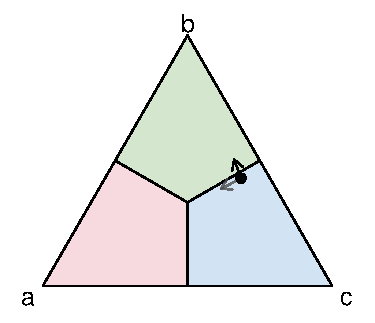
\includegraphics[width=0.33\textwidth]{./../../output/figs/20190423/plurality_illustration.pdf} & 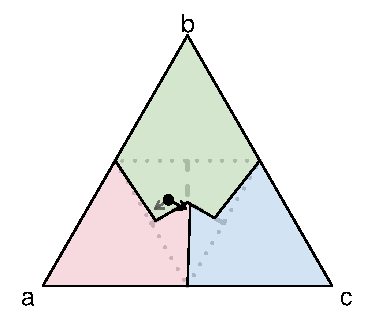
\includegraphics[width=0.33\textwidth]{./../../output/figs/20190423/irv_illustration_1.pdf} & 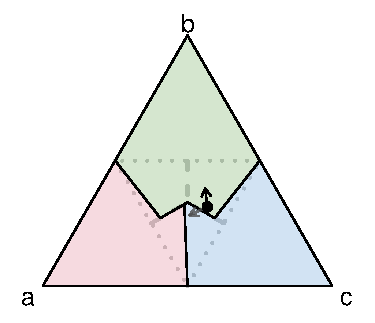
\includegraphics[width=0.33\textwidth]{./../../output/figs/20190423/irv_illustration_2.pdf}
\end{tabular} 
\end{center} 
\footnotesize{Note: There is one type of strategic voting incentive in plurality and two types in IRV. The ternary diagrams above depict a situation in which a voter with sincere preference $abc$ might strategically vote $b$ (left), $cab$ (center), or $bac$ (right). See \citet{eggersternary} for more on the use of ternary diagrams to represent IRV election results.} 
\end{figure} 


%\begin{comment} 
%  voter optimally abandons a trailing candidate in a plurality election clearly depends on the voter's beliefs about the election result. Conditional on the distribution of sincere preferences in the electorate, the expected result depends on voters' strategies. If voters agree about  
%
%Given information about other voters' sincere preferences (e.g.\ from a poll), beliefs about the election result depends on beliefs about other voters' voting strategies 
%
% on what the voter expects other voters to do: the more she expects other voters to desert this candidate, the more likely it is that she should also desert the candidate. On the ternary diagram, as voters with sincere preference $abc$ and $acb$ desert candidate $a$, the expected result moves to the northeast (away from $a$'s vertex); for a reasonable specification of uncertainty (e.g.\ a Dirichlet distribution) this reduces the probability of an $ab$ or $ac$ tie relative to a $bc$ tie, which makes an insincere vote optimal for a larger set of $a$-preferring voters.        %formalize/depict this? 
%Thus desertion of a trailing candidate in plurality elections tends to snowball: put differently, one voter's decision to desert a trailing candidate or not is a strategic complement to another voter's decision to desert that candidate or not. \emph{TODO: consider private info/Myatt point. Formalize the prevalence/magnitude distinction? Also, strategic substitutes when I am deciding whether to desert $a$ and you are deciding whether to desert $b$.} If voters respond strategically to a public poll, for example, we should expect fewer voters to cast sincere votes when the public poll   
%
%strategic voting incentives in plurality elections are higher when the expected result .   
%
%\end{comment} 

\subsubsection{IRV} 

\noindent \textbf{Preliminaries}  The logic of strategic voting is more complex in an IRV election. To describe that logic, we will discuss a three-candidate IRV election as if it took place in two rounds: a first round in which the candidate with the fewest first-place votes is eliminated and a second round in which the winner is determined based on which of the remaining candidates is ranked higher on more ballots. A single vote can determine the winner at either stage: it can be \emph{first-round pivotal} by determining which candidate is eliminated and thereby affecting which candidate wins, and it can be \emph{second-round pivotal} by determining which of the non-eliminated candidates is elected.\footnote{Technically it can also determine whether a candidate receives an outright majority of first-place rankings, but we can safely ignore these pivotal events because a candidate who is one vote away from winning an outright majority of first-place rankings could only lose the election if that candidate is not ranked second on any ballots that ranked the eliminated candidate first, which is unlikely in a large electorate.} 

In total there are twelve pivot events in a three-candidate IRV election. % (compared to three in a plurality election). 
There are three scenarios in which a single ballot could determine the winner given that two candidates (say, $a$ and $b$) are tied in the first round: % pair of candidates is tied in the first round (say, $a$ and $b$), then there are three scenarios in which a single ballot could determine the winner: 
$c$ would lose to either $a$ or $b$ in the second round, $c$ would lose to $a$ but not $b$, or $c$ would lose to $b$ but not $a$. (If $c$ would not lose to either $a$ or $b$, then it is not a pivot event, as the winner does not depend on a single vote.) Thus for each of three pairs of candidates there are three first-round pivot events, for a total of nine first-round pivot events. Each pair of candidates can also be tied in the second round (e.g.\ $c$ finishes last in the first round and, after $c$'s votes are redistributed, $a$ and $b$ have the same level of support), for a total of three second-round pivot events and a grand total of twelve pivot events. 

In principle we need to consider six possible ballots for each voter: $abc$, $acb$, $bac$, $bca$, $cab$, and $cba$.\footnote{If incomplete rankings are permitted, as they are in many Australian state legislative elections, then voters could also submit a ballot that ranks only two candidates ($ab$, $ac$, $ba$, $bc$, $ca$, and $cb$) or a ballot thats rank only one candidate ($a$, $b$, $c$), but for computing the optimal ballot we can ignore these incomplete rankings. If, when candidate e.g.\ $a$ is eliminated, ballots listing $a$ first are transferred to the candidate ranked second on those ballots, then a ballot ranking all but one candidate (e.g.\ $ab$) has the same effect on outcomes as a ballot that includes the omitted candidate at the end (e.g.\ $abc$), so we can consider those ballots as equivalent. If voters have strict preferences over candidates and all pivotal events have non-zero probability, then a ballot ranking only one candidate is strictly worse than a ballot ranking that candidate first followed by the voter's sincere ranking of the remaining candidates (because a second-round tie between those candidate is possible), so ranking a single candidate is never optimal. \citet{fishburn1984manipulability} showed that submitting a truncated ballot can be better than submitting a sincere ballot when there are four or more candidates, essentially because it avoids the no-show paradox, but even then another non-truncated ballot must be optimal.}  In fact for any given voter we can focus on just three possible ballots.\footnote{\citet[][p.~224]{dummett1984voting} makes this point.} To see why, note first that in any first-round pivot event the outcome depends only on one's top ranking, and as we will see shortly there are circumstances in which a voter benefits from giving the top ranking to her true first, second, or third choice. There is no reason to insincerely rank the other two candidates, however: these lower rankings are irrelevant in first-round pivot events and, when they matter for second-round pivot events, can only backfire if they do not reflect the voter's sincere preference. In short, whatever candidate one ranks first, one should rank the other two sincerely in case those candidates are tied in the second round. %\footnote{Dummett makes this point too. TODO: cite} 
For each voter, then, the question is whether to give the top ranking to $a$, $b$, or $c$, with the lower rankings following the voter's sincere preference; for example, a voter with sincere preference $abc$ should consider voting $abc$, $bac$, or $cab$ but can ignore $acb$, $bca$, or $cba$. \\
%  We will therefore sometimes use the shorthand ``vote for $a$'' when we mean ``rank $a$ first, with lower rankings following the voter's sincere preference''. 

\noindent \textbf{Qualitative characterization} In contrast to plurality, where there is one type of strategic voting incentive (which we described above as ``abandoning a trailing candidate to avoid wasting one's vote''), in IRV there are two basic types of strategic voting incentive. The first type can be described as ``abandoning a \emph{leading} candidate to avoid wasting one's vote''. This incentive arises when one's first choice, $a$, is expected to safely advance to the second round, but a tie for second between $b$ and $c$ is possible, such that by voting $bac$ or $cab$ one can determine whether $b$ or $c$ advances to the second round. 
%(If $b$ and $c$ tie for second in the first round, a sincere $abc$ vote does not .) 
Abandoning a leading candidate (here, $a$) is beneficial either when $b$ and $c$ would both defeat $a$ in the second round (in which case voting $bac$ or $cab$ determines whether $b$ or $c$ is elected) or when $a$ would beat one candidate (say, $c$) but not the other (in which case voting $cab$ secures $a$'s election). 

The second type of strategic voting incentive in IRV can be described as ``abandoning a trailing candidate to avoid electing one's least favorite candidate''. This incentive arises when one's last choice ($c$) is expected to finish first in the first round, and one's second choice ($b$) can defeat $c$ in the second round while one's first choice ($a$) cannot. (This might be the case if, for example, $a$, $b$, and $c$ were arranged left to right on a single policy dimension, with $b$ as the centrist and Condorcet winner.) If $a$ and $b$ were to tie for second, then a sincere $abc$ vote would cause $a$ to eliminate $b$, leading to the election of $c$, while a $bac$ vote would cause $b$ to advance and defeat $c$. By contrast with the strategic voting incentive in plurality, one abandons a trailing candidate here not because one's vote is \emph{wasted}, but rather because it \emph{backfires}; indeed, in this scenario one would be better off not voting than voting sincerely (which is why systems that produce this incentive are said to suffer from the ``no-show paradox'').\\

\noindent \textbf{Visualization} Following \citet{eggersternary} we extend the ternary diagram in Figure \ref{fig:three_types} to depict the two types of strategic voting incentives in IRV elections. The axes of the IRV ternary diagrams indicate the proportion of ballots ranking each candidate first. As in the plurality case, the triangle is divided into regions in which each candidate wins; unlike in the plurality case, the boundaries depend on the proportion of ballots ranking each candidate second conditional on which candidate is ranked first. In the IRV diagrams in Figure \ref{fig:three_types}, the pattern of preferences is roughly single-peaked, with $b$ as the centrist candidate.\footnote{See \citet{eggersternary} for more on the construction and interpretation of the ternary diagram for IRV.} Near the center of the diagram, the bottom boundary of $b$'s win region follows an upside-down $V$ shape. At results along the left branch of the upside-down V (highlighted in the center diagram), there is a tie for second between $b$ and $c$ in the first round, and $b$ would win the election if $b$ advanced while $a$ would win the election if $c$ advanced. For a voter with sincere preference $abc$, a result like this provokes the first type of IRV strategic voting incentive: a sincere $abc$ vote would move the result toward $a$'s vertex (as indicated by the gray arrow) but would not affect the winner, while a $cab$ vote would move the result into $a$'s win region (as indicated by the black arrow). At results along the right branch of the upside-down V (highlighted in the right diagram), there is a tie for second between $a$ and $b$ in the first round, and $b$ would win the election if $b$ advanced while $c$ would win the election if $a$ advanced. For a voter with sincere preference $abc$, a result like this provokes the second type of IRV strategic voting incentive: a sincere $abc$ vote would move the result into $c$'s win region, while a $bac$ vote would move the result more safely into $a$'s win region. \\

\subsection{Dependence of strategic voting incentives on the level of strategic voting}

Suppose a poll takes place in which voters are asked for their sincere ratings of competing candidates. What should a strategic voter believe about likely election results, given this polling information? Clearly the appropriate belief depends on the extent to which other voters are strategic and how these voters form their beliefs about likely election results. If other voters are completely non-strategic, the poll offers a good direct approximation of the likely election result; if other voters are themselves strategic, a strategic voter can only form a belief about likely results by first forming a belief about how others use the poll to form a belief. As discussed above, our analysis posits that voters have a range of levels of rationality; we examine strategic voting incentives for a sequence of beliefs as voters are perceived to become more strategic. 
%our approach to characterizing expectations as others are perceived to become more beliefs is to trace out a sequence of election outcomes from sincerity toward a (possible) strategic voting equilibrium; the stages of this sequence can be seen as the beliefs of voters who posit  successively higher levels of rationality in the electorate. 
For now, we seek only to develop intuition about how strategic voting incentives depend on beliefs about others' strategic orientation and why this differs in plurality and IRV elections; to do this, it is sufficient to compare the incentives of level-1 and level-2 voters (i.e.\ those who believe that other voters are non-strategic and those who believe that some other voters are level-1) and observe how this comparison differs between the plurality case and the IRV case.  
% focus only on the first step of this sequence: how does the incentive to vote strategically differ between level-1 and level-2 voters, and how does this difference vary between plurality and IRV elections?

To begin, it is useful to note that the strategic voting incentive (i.e.\ the average difference in expected utility between a strategic vote and a sincere vote) can be decomposed into two parts, which we will call \emph{prevalence} and \emph{magnitude}: 
\[
\underbrace{E\left[\overline{u}(b^*) - \overline{u}(b_s)\right]}_{\text{Exp.\ benefit of strategic voting}} = \underbrace{\text{Pr}\left( \overline{u}(b^*) > \overline{u}(b_s)\right)}_{\substack{ \text{ Prob.\ tactical vote optimal} \\ \textbf{(prevalence)}} } \times \; \, \underbrace{E\left[ \overline{u}(b^*) - \overline{u}(b_s) \mid \overline{u}(b^*) > \overline{u}(b_s)\right]}_{\substack{\text{Avg.\ benefit of an optimal tactical vote} \\ \textbf{(magnitude)}}}.
\]   
% \\ (diff in exp.\ utility btw strat.\ vote and sincere vote)}
We focus in this section on the prevalence term; there is more ambiguity in how the magnitude of strategic voting incentives depends on beliefs about others' strategies. Our objective is to understand how the prevalence of strategic voting benefits depends on how strategic other voters are expected to be.
  
We begin with plurality. Recall that  strategic voting in plurality elections involves abandoning candidates who are not expected to be in contention for first place. Level-1 voters expect the election result to resemble the poll in expectation. Given Dirichlet beliefs and three candidates, therefore, some level-1 voters abandon the candidate with the lowest sincere support;\footnote{Others may abandon the candidate with the second-lowest sincere support.} the decision depends on belief precision and strength of relative preferences. If level-2 voters expect the election result to be a weighted average of the poll and the best responses of level-1 voters, and if strategic responses by level-1 voters make the candidate with the lowest sincere support even less competitive,\footnote{This is not guaranteed because of desertions from the candidate with the second-lowest sincere support. For example, strategic votes by level-1 voters could reverse the expected order of finish of the sincere second- and third-place candidates, such that the candidate with the lowest sincere support is seen as more competitive by level-2 voters.} then the prevalence of strategic voting benefits (i.e.\ the proportion who optimally cast as insincere vote) should be higher among level-2 voters than level-1 voters. Because the incentive to desert an unpopular candidate tends to become more widespread when others are expected to desert that candidate, strategic voting in plurality elections is characterized by \emph{strategic complementarity}: if others desert a trailing candidate, I am more likely to benefit from deserting that candidate.

In IRV the situation is different. Suppose that (as above) $a$ is the left-wing candidate, $b$ is the centrist candidate, and $c$ is the right-wing candidate, and suppose that $c$ has the largest share of sincere first-preferences. Given level-1 beliefs, a voter with $cba$ preference order has an incentive to submit a $acb$ ballot to help the weaker opponent, $a$, advance to the second round. ($a$ is expected to be the weaker opponent because $a$ is listed second on only some of $b$'s ballots while $b$ is listed second on all of $a$'s ballots.) For the same reason, a voter with $abc$ preference order has an incentive to submit a $bac$ ballot to avoid the situation where $a$ eliminates $b$, electing $c$. (These are examples of the two strategic voting incentives in IRV.) Given level-2 beliefs, however, these incentives will be more limited. The incentive for $cba$ types to vote $acb$ is reduced in part because, as more voters desert the leading candidate to avoid wasting their vote, that candidate's lead becomes less secure. More subtly, both incentives are reduced because the strategic votes of type-1 voters, prompted by $a$'s weakness relative to $b$ as an opponent for $c$, tend to make candidate $a$ \emph{stronger} relative to $b$ as an opponent to $c$, thus producing negative feedback. To see this, note that both $cba \rightarrow acb$ votes and $abc \rightarrow bac$ votes tend to increase the proportion of votes for $a$ that list $c$ second, and $abc \rightarrow bac$ votes tend to increase the proportion of votes for $b$ that list $a$ second. This diminishes the discrepancy that motivated these votes in the first place: as a result of these strategic moves, and conditional on a tie for second between $a$ and $b$ in the second round, $a$ is a stronger potential opponent for $c$ (because more of $b$'s ballots list $a$ second) and $b$ is a weaker potential opponent for $c$ (because more of $a$'s ballots list $c$ second). The general pattern in IRV is that, when voters strategically respond to a discrepancy between the second preferences of two candidates (here, $b$'s second preferences being more favorable to $c$ than $a$'s are), this discrepancy tends to disappear.  Because both incentives in IRV tend to diminish when others are expected to act on them, strategic voting in IRV elections is characterized by \emph{strategic substitutability}: if others desert a leading candidate to avoid wasting a vote or desert a trailing candidate to avoid electing their least favorite candidate, I am less likely to follow suit.\footnote{There are exceptions. For example, deserting a leading candidate who cannot defeat either candidate in the second round can exhibit strategic complementarity: the less support the candidate gets, the more important it is to determine which other candidate advances. This incentive, too, must eventually attenuate, however, as the candidate becomes less and less likely to advance.}

% We now turn to the magnitude of strategic voting benefits, i.e.\ how much one expects to benefit from strategic voting conditional on an insincere vote being optimal. How does this differ for level-1 and at level-2 voters? Supposing that level-1 voters abandon the trailing candidate, such that this candidate is even less competitive,      

\section{Data}

To assess the prevalence and distribution of strategic incentives under Plurality and IRV empirically, we rely on data from the  Comparative Study of Electoral Systems (CSES) for a realistic set of preferences and beliefs. The dataset covers 160 surveys from xx different countries, administered shortly before or after an election.\footnote{Two additional cases in the survey, Belarus (20xx) and Lithuania (20xx), are dropped because no respondent specified full preferences over more than two parties.} We focus on the three largest parties (evaluated how?) and label them $A, B, C$ in descending size, respectively. From each survey in the data set, we take respondents' party like/dislike scores for these parties to approximate voters' ordinal utilities and, by extension, their preferences over the parties.

Let $\bf \tilde{v}$ be the vector of ballot proportions if everyone in the CSES survey voted sincerely according to their preferences. If voter $i$ believes that everyone else is voting sincerely (in other words, everyone else is Level-0 strategic), then we model the $i$'s belief about the next election as $\text{Dir}(s \times \bf \tilde{v})$, where $s$ is a parameter capturing the precision of $i$'s beliefs. Given this set-up of beliefs and preferences, we calculate the strategic incentives under either electoral system, and iterate this procedure as laid out in Section 3.

The remainder of this section describes brief summary statistics of the CSES data.


\subsection{Summary statistics}

\begin{figure}[!htb]
	\centering
	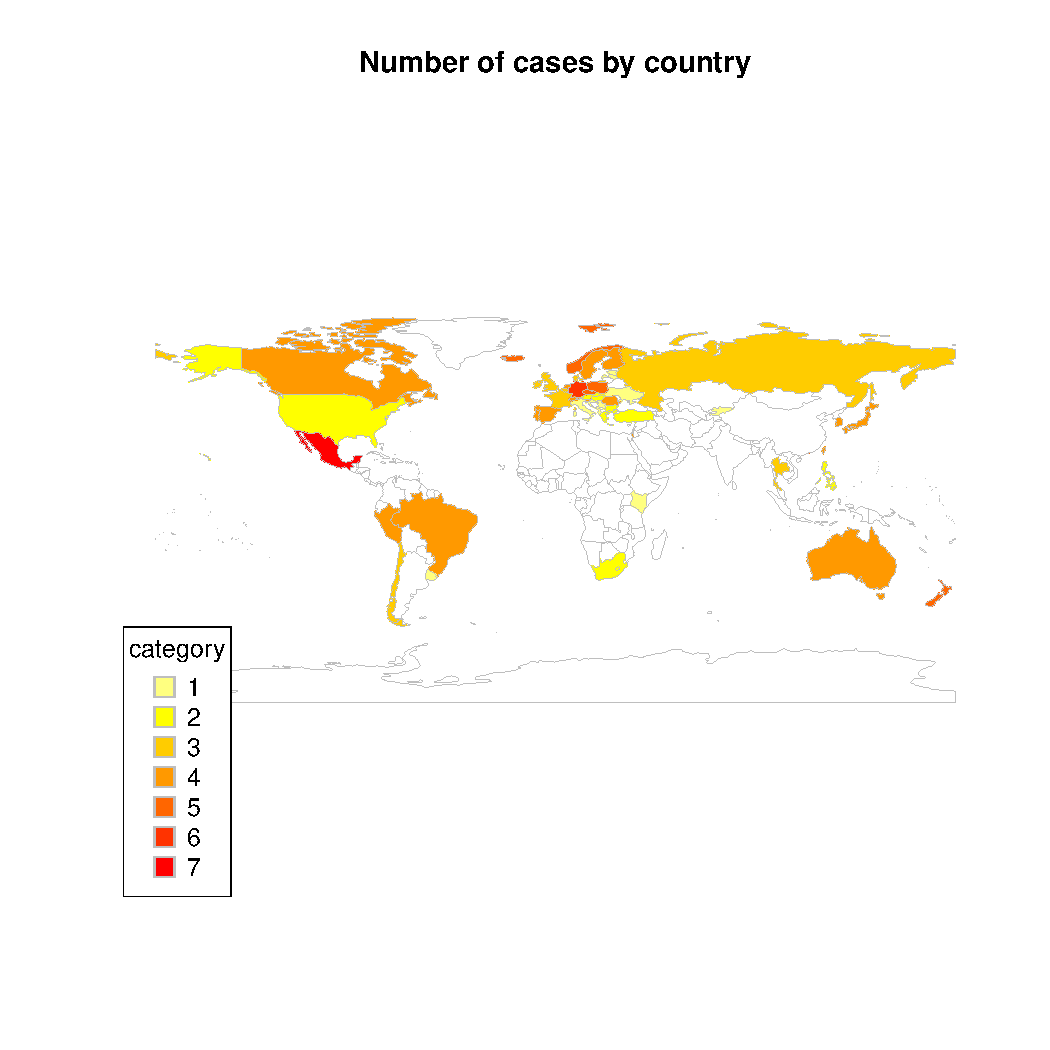
\includegraphics[width = .5 \textwidth]{../../output/figures/case_map.pdf}
	\caption{Cases in CSES data, by country}
	\label{fig:case_map}
\end{figure}

The mean number of respondents in the CSES surveys is 1384 (with a standard deviation of 539). The 160 different surveys come from xx different countries, between 1996 and 2016. Figure~\ref{fig:map} maps the number of surveys in each country. (Do we need to say any more? Perhaps something about mean / sd of preference intensity and $\tau$?)

\subsection{Weighting}

In some CSES cases, respondents are assigned a non-uniform weight. When computing case-level statistics (e.g., prevalence of strategic incentives in case $j$), we weigh each observation by its original weight. When aggregating up even further, and presenting aggregate statistics (averaged over all cases), we also assign case-level weights to adjust for countries' voting age population and the overrepresenation of some countries.\footnote{Recall that our initial objective is to compare the \textit{overall} distribution of strategic voting incentives under Plurality and IRV. Without weights, we would run the risk of having our findings distorted by a small countryoutlier that counts for as much as a large state (e.g., Denmark and the United States); alternatively, we also do not want a result that is particular to one country to be over-represented purely because there are multiple surveys from that country.}

These case-level weights are constructed as follows:

\begin{equation}
	w_j \equiv
\end{equation}

\subsection{Distribution of preferences} 

How different are the CSES cases from one another? Aside from the intensity of preferences, we can describe each case with the vector $\bf \tilde{v}$, where the three-item vector $(v_1 + v_2, v_3 + v_4, v_5 + v_6)$ describes the distribution of first preferences, and the three-item vector $(m_{AB} = \frac{v_1}{v_1 + v_2}, m_{BA} = \frac{v_3}{v_3 + v_4}, m_{CB} = \frac{v_6}{v_5 + v_6})$ describes the distribution of second preferences. 

To link these two distributions together and classify cases more completely, we offer the following approach. Without loss of generality, let the candidate (party) $X$ whose first-preference voters have the most equally split second preferences, and the other two parties $Y$ and $Z$. If both $m_{YZ}$, $m_{ZY} > 0.6$, then classify this case as \emph{single-peaked} and denote it $X+$.\footnote{$X$ is the attractor: both remaining parties have a majority of their second preferences tilted towards $X$.} Conversely, if both $m_{YZ}, m{ZY} < 0.4$, then classify this case as \emph{divided majority} and denote it $X-$.\footnote{Here, $X$ is the repeller: both remaining parties have a majority of their second preferences tilted towards each other and away from $X$.} If $m_{YZ}, m_{ZY} \in [0.4, 0.6]$, then classify this case as \emph{neutral} and denote it $N(X)$. If neither of these conditions hold (because of unusual second preferences), classify it as \emph{other} and denote it $O$. This completes a mutually exclusive and exhaustive set of classes determined by $\bf \tilde{v}$.

\begin{table}[tb]
	\caption{Distribution of preference profiles in CSES data}
	\label{tab:csesprefs}
	\centering

	\begin{tabular}{lccc}
	\hline

	\toprule
	\textbf{} & \textbf{A} & \textbf{B} & \textbf{C} \\
	\cmidrule{2-4}
	Single-peaked (+) & 18 & 23 & 9  \\
	Divided majority (-) & 28 & 20 & 20  \\
	Neutral () & 5 & 7 & 3  \\
	Other () & & 27 &  \\
	\bottomrule
	\end{tabular}
\end{table}

Table~\ref{tab:csesprefs} summarises the distribution of preference classes across the CSES cases. A plurality of cases belong to the divided majority classes; however, there is also a large number of single-peaked cases, whereas neutral and others tend to be rarer. (Figure~\ref{fig:cses_fp} plots the distribution of first preferences conditional on the classes.)

\begin{figure}[!htb]
	\centering
	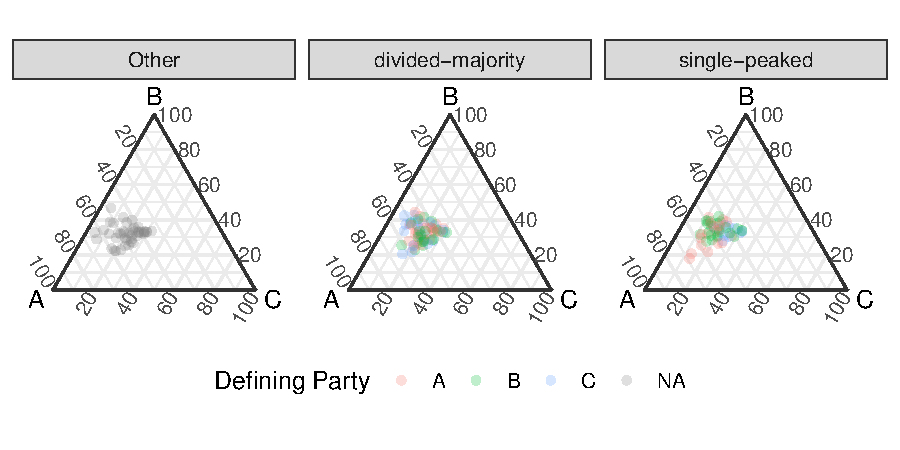
\includegraphics[width = 0.6 \textwidth]{../../output/figures/cses_fp.pdf}
	\caption{Distribution of first preferences in CSES cases, by class}
	\label{fig:cses_fp}
\end{figure}

\section{Results}

We now proceed to present and discuss our results.

\subsection{Convergence}

Under both IRV and Plurality, the distribution of ballot shares quickly converges towards a fixed point in the vast majority of CSES cases. The average Euclidean distance going from the 59th to the 60th iteration is below 0.0014 for Plurality, and below 0.006 for IRV.\footnote{These averages are unweighted -- need to recompile in the future.} Put differently, we can obtain a perfectly strategic voting equilibrium, where all voters anticipate others' vote choices, and react accordingly, within about 60 iterations from the sincere voting profile.

\begin{figure}[!tbh]
	\centering
	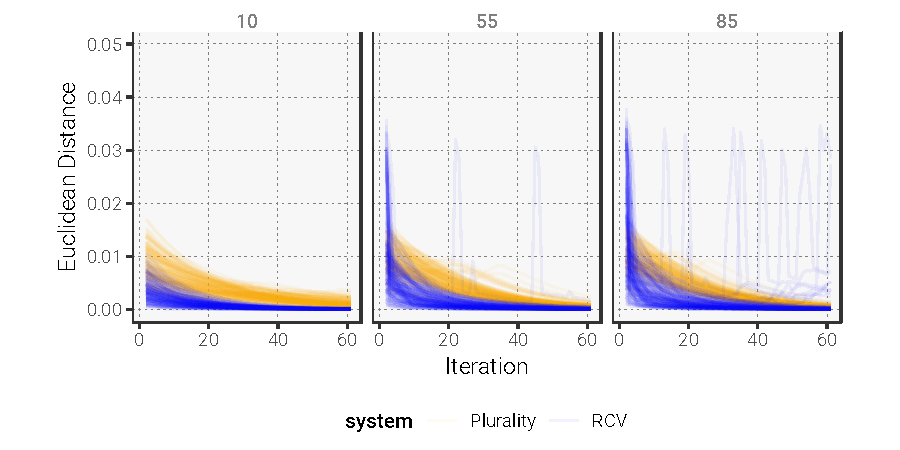
\includegraphics[width = \textwidth]{../../output/figures/euclidean}
	\caption{Euclidean distance between ballot share vectors from one iteration to another.}
	\label{fig:convergence}
\end{figure}

Figure~\ref{fig:convergence} plots the Euclidean distance between the ballot shares for every case and iteration under both Plurality and IRV. In expectation, convergence towards the fixed point occurs faster under IRV than it does under Plurality. As we discussed earlier, strategic incentives under Plurality are characterised by complementarity; this means that with every additional iteration, the incentive for supporters of the third party increases, until all of them have deserted the trailing candidate and the ballot shares are in a Duvergian (two-party) equilibrium.\footnote{We could visualise this by plotting the share of third-party votes when $k = 60$.} In contrast, the substitutability of strategic voting incentives under RCV allows them to reach a fixed point much sooner. Note however, that, for more precise beliefs ($s \in {55, 85}$), the shift away from the sincere ballot profile in the first few iterations is much bigger than under Plurality; quicker convergence does not necessarily mean that the fixed point is closer to the original ballot share vector.\footnote{This foreshadows a later result: with sufficiently high precision, the prevalence of strategic voting incentives under IRV will be higher in the first few incentives.}

In sum, when applying our iterative strategic voting procedure to all CSES cases, the ballot shares converge more quickly to a fixed point under IRV than under Plurality. Under IRV, these fixed points can occur anywhere in the ballot share space, whereas under Plurality, voters ultimately settle on a two-party Duvergian equilibrium. This is also illustrated by Figure~\ref{fig:convergence_paths}, which maps the ballot share vectors before the first and the 60th iteration for $s = 85$.

(Figure about distance from sincere profile? -- shows nicely that Plurality fixed points are further away from initial ballot shares.)

\begin{figure}[]
	\centering
	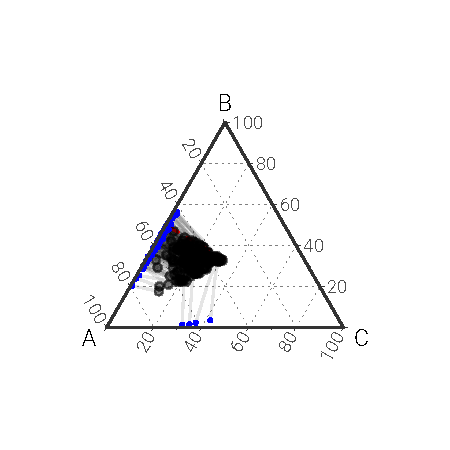
\includegraphics[width = .49\textwidth]{../../output/figures/tatonnement_plur}
	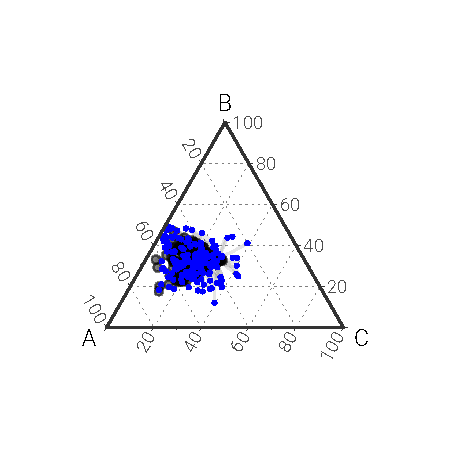
\includegraphics[width = .49\textwidth]{../../output/figures/tatonnement_rcv}
	\caption{Evolution of ballot share vectors for all CSES cases over iterations, for both Plurality (left) and IRV (right), when $s = 85$. Grey dots indicate the initial ballot share vector before the first iteration; blue dots the ballot share vector after the 60th iteration.}
	\label{fig:convergence_paths}
\end{figure}

\subsection{Strategic Incentives}

In this section, we present our main results. We focus on the prevalence, magnitude and expected benefit of strategic voting under either electoral system. Overall, strategic voting incentives are more prevalent, have a higher magnitude and higher expected benefit under Plurality than under IRV.

Figure~\ref{fig:main_stats} shows the quantities of interest for each case, as well as the weighted average.

\begin{figure}[]
	\centering
	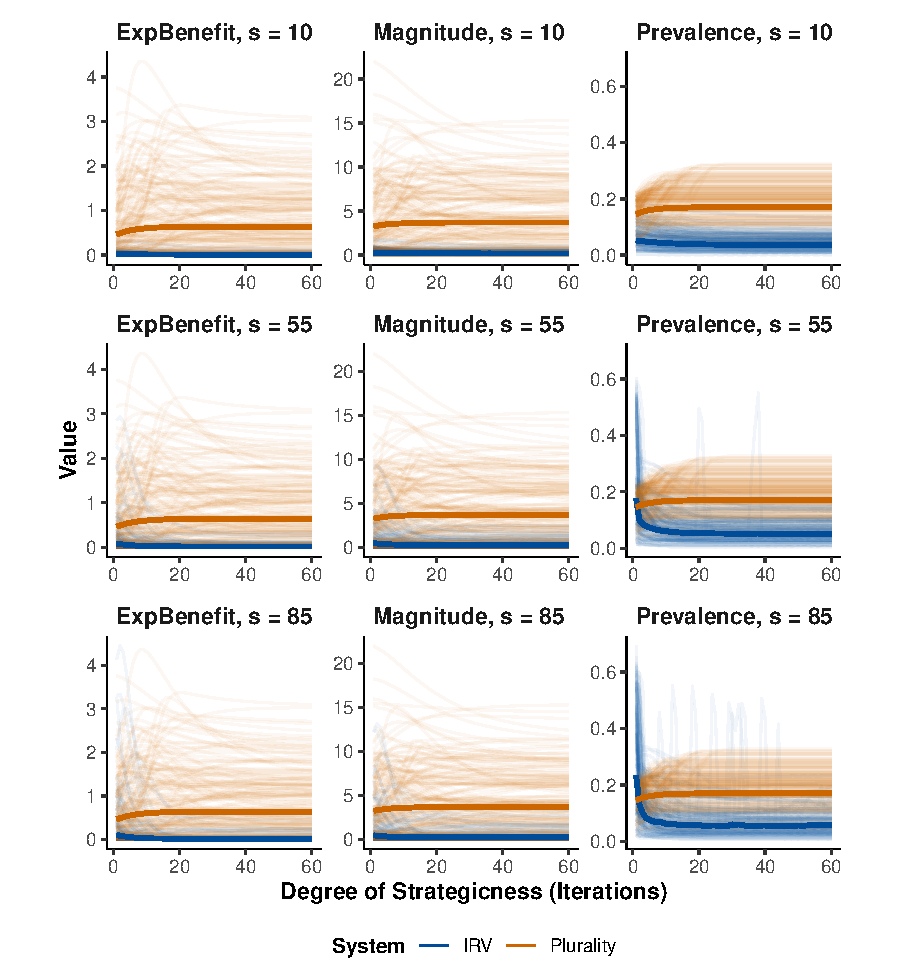
\includegraphics[width = \textwidth]{../../output/figures/iterated_complete}
	\caption{Main statistics}
	\label{fig:main_stats}
\end{figure}

\section{Conclusion}




\newpage 

\bibliographystyle{apsr}
\singlespacing
\bibliography{./../strategic_voting}


\newpage 


\appendix 



\section{The probability of pivotal events in IRV elections} 

% \emph{\textsc{Note:} The material below needs a lot of work and may need to be in its own paper in some form. For now let's plan on this being in an appendix in this paper, and perhaps another paper follows. At a minimum revisions to this appendix must deal with (i) introducing pivotal events; (ii) harmonizing notation; (iii) deciding whether to focus on standard Dirichlet beliefs only, or two-level sampling; (iv) whether to include truncated rankings or not; (v) identifying and fixing error AE detected and noted in an email to TN when second preferences are very skewed (can see it when we relabel candidates and get very different answers).}

% \subsection{Preliminaries} 

Given beliefs about the likelihood of possible election outcomes, the probability of pivotal events (i.e.\ results such that the outcome could be affected by a single ballot) can be calculated either by a numerical/analytical method involving integration of the belief distribution or by a simulation method. This section presents both approaches (beginning with the numerical/analytical method) and shows that they produce the same result, though the simulation method is much more computationally intensive. \\    

\noindent \textbf{Ballots}: In an IRV election with three candidates $\{a,b,c\}$ in which all ballots must rank all candidates,\footnote{The analysis can be extended to allow truncated ballots.} there are six admissible ballots. Let $v_{ab}$ denote the share of ballots ranking candidate $a$ first, $b$ second, and (implicitly) $c$ third (with $v_{ac}$, $v_{ba}$, etc.\ defined equivalently). Then the vector of ballot shares is 
\[
\mathbf{v} = \{ v_{ab}, v_{ac}, v_{ba}, v_{bc}, v_{ca}, v_{cb} \}. 
\]  
Let $v_a \equiv v_{ab} + v_{ac}$ denote the share of ballots ranking candidate $a$ first (with $v_b$ and $v_c$ defined equivalently); we will refer to $v_a$, $v_b$, and $v_c$ as \emph{first-preference shares}. Finally, let $\overline{v}_{ab}$ denote the expected share of ballots ranking $a$ first and $b$ second, with $\mathbf{\overline{v}}$ indicating the vector of expected ballot shares (and $\overline{v}_{ac}$, $\overline{v}_{ba}$, etc.\ defined equivalently) and let $\overline{v}_{a} \equiv \overline{v}_{ab} + \overline{v}_{ac}$ (with $\overline{v}_b$ and $\overline{v}_c$ defined equivalently). \\

\noindent \textbf{Pivotal events}: There are two broad classes of pivotal results in a three-candidate IRV election. %  which we will refer to as \emph{first-round pivotal events} and \emph{second-round pivotal events}. 
In a \emph{first-round pivotal event}, two candidates tie for second place in first-preference shares, and the identify of the winner depends on which candidate is eliminated. Let $ab.ab$ denote the first-round pivotal event in which $a$ and $b$ tie for second place in first-preference shares and $a$ wins the election if $a$ advances while $b$ wins the election if $b$ advances; similarly, let $ab.ac$ denote the first-round pivotal event in which $a$ and $b$ tie for second place and $a$ wins the election if $a$ advances while $c$ wins the election if $b$ advances; let $ab.cb$ denote the first-round pivotal event in which $a$ and $b$ tie for second place and $c$ wins the election if $a$ advances while $b$ wins the election if $b$ advances. Let $ac.ac$, $ac.ab$, $ac.bc$, $bc.bc$, $bc.ba$, and $bc.ac$ be defined similarly.  In a \emph{second-round pivotal event}, two candidates tie after the other candidate is eliminated; let $ab$ denote the second-round pivotal event involving $a$ and $b$, with $ac$ and $bc$ defined similarly. We will denote the probability of pivotal event e.g.\ $ab$ by $\pi_{ab}$.\\

\noindent \textbf{Beliefs}: We assume that election outcomes are believed to follow a Dirichlet distribution centered on $\overline{\mathbf{v}}$ with precision captured by $\gamma$, i.e.\ 
\begin{equation}
\mathbf{v} = \{v_{ab}, v_{ac}, v_{ba}, v_{bc}, v_{ca}, v_{cb} \} \sim \mathrm{Dir}(\alpha_{ab}, \alpha_{ac}, \alpha_{ba}, \alpha_{bc}, \alpha_{ca}, \alpha_{cb})  \label{dirichlet}
\end{equation}
where e.g.\ $\alpha_{ab} = \gamma \overline{v}_{ab}$. We will make use of three well-known \citep{frigyik2010introduction} properties of the Dirichlet distribution:

%Let the random variable $\pi = (\pi_1, \pi_2, \ldots, \pi_k)$ be a vector of vote shares that follows a Dirichlet distribution with parameter $\alpha = (\alpha_1, \alpha_2, \ldots, \alpha_k)$. That is, $(\pi_1, \pi_2, \ldots, \pi_k) \sim  \text{Dir}\big(\alpha_1,\alpha_2, \ldots, \alpha_k\big)$.  
%We will make use of three well-known \citep{frigyik2010introduction} properties of the Dirichlet distribution:

\smallskip

\noindent \emph{Aggregation property}: $(v_1, v_2, \ldots, v_i + v_j, \ldots v_B) \sim  \text{Dir}\big(\alpha_1,\alpha_2, \ldots, \alpha_i + \alpha_j, \ldots \alpha_B\big)$. (If two of the vote shares are added together to create a new, shorter vector of vote shares, the new vector of vote shares also follows a Dirichlet distribution, where the parameters corresponding to the summed-up vote shares are also summed up.)

\smallskip

%\noindent In words, if two of the vote shares are added together to create a new, shorter vector of vote shares, the new vector of vote shares also follows a Dirichlet distribution, where the parameters corresponding to the summed-up vote shares are also summed up. 

%\smallskip 

\noindent \emph{Marginal distribution}: $v_i \sim \text{Beta}(\alpha_i, \sum_{-i} \alpha)$.  (Unconditionally, any particular vote share follows a Beta distribution. This follows from the aggregation property and the observation that a Dirichlet distribution with two parameters is a Beta distribution.)

\smallskip
%\noindent Unconditionally, any particular vote share follows a Beta distribution. 
% \smallskip 
\noindent \emph{Conditional distribution}: $(v_1, \ldots, v_{i -1}, v_{i+1}, \ldots, v_B \, | \, v_i) \sim (1 - v_i) \text{Dir}(\alpha_1, \ldots, \alpha_{i -1}, \alpha_{i+1}, \ldots, \alpha_B)$.   (Conditional on $i$ receiving share $v_i$, the remaining shares follow a rescaled Dirichlet distribution in which $\alpha_i$ is removed from the parameter vector.)
\begin{comment} 
It follows from the aggregation property that first-preference shares are also distributed according to a Dirichlet, i.e.\ 
\begin{eqnarray} 
(v_a, v_b, v_c) &\sim&  \mathrm{Dir}(\gamma \overline{v}_{ab} + \gamma \overline{v}_{ac}, \gamma \overline{v}_{ba} + \gamma \overline{v}_{bc}, \gamma \overline{v}_{ca} + \gamma \overline{v}_{cb}) \nonumber \\
&=&  \mathrm{Dir}(\gamma \overline{v}_a, \gamma \overline{v}_b, \gamma \overline{v}_c). \nonumber
\end{eqnarray} 
\end{comment} 
%\begin{equation} 
%(v_a, v_b, v_c) \sim  \mathrm{Dir}(\gamma \overline{v}_{ab} + \gamma \overline{v}_{ac}, \gamma \overline{v}_{ba} + \gamma \overline{v}_{bc}, \gamma \overline{v}_{ca} + \gamma \overline{v}_{cb}) = \mathrm{Dir}(\gamma \overline{v}_a, \gamma \overline{v}_b, \gamma \overline{v}_c). \nonumber
%\end{equation} 

%Note that a Dirichlet distribution with only two share components is equivalent to a Beta distribution. Thus it also follows from the aggregation property that 
%\begin{eqnarray} 
%v_a &\sim&  \mathrm{Dirichlet}(v_a, v_b + v_c; \gamma \overline{v}_{a}, \gamma (\overline{v}_b + \overline{v}_c)) \nonumber \\
%&=&  \mathrm{Beta}(v_a; \gamma \overline{v}_{a}, \gamma (\overline{v}_b + \overline{v}_c)). \nonumber
%\end{eqnarray}  

We will use $f(\mathbf{v}; \gamma \overline{\mathbf{v}})$ to indicate the Dirichlet density with parameters $\gamma \overline{\mathbf{v}}$ evaluated at $\mathbf{v}$. Because the Beta density can be seen as a special case of the Dirichlet density, we will use $f(\cdot)$ for both.\\  % is Note that a Dirichlet distribution with only two share components is equivalent to a Beta distribution. (The Dirichlet distribution can be seen as a generalization of the Beta distribution.) \\ 
%We will use $f(\cdot)$ 
%  because the Beta density can be seen as a special case of the Dirichlet density, we will not distinguish between them.\\   

\noindent \textbf{Probability of second-round pivotal events}: 
If we say that two candidates tie when their vote share differs by less than half a vote,\footnote{This is equivalent to saying that we calculate the probability of specific results by rounding continuous vote shares to the closest multiples of $1/N$.} 
% receive the same number of votes, and if we assume that the probability of this is equal to the probability that their vote share differs by less than half a vote (which is strictly positive given our simplifying assumption that vote shares are viewed as continuous),    
then the probability of second-round pivotal event $ab$ can be written 
\begin{equation}   \text{Pr}\left( v_c < v_a < \frac{1}{2}  \cap   v_c < v_b < \frac{1}{2} \cap v_a + v_{ca} - \frac{1}{2} \in \left(-\frac{1}{2N}, \frac{1}{2N} \right) \right).  \nonumber \end{equation} This can be factorized as  
%The probability of second-round pivotal event $ab$ can be written 
\begin{equation}  \text{Pr}\left(v_a + v_{ca} - \frac{1}{2} \in \left[-\frac{1}{2N}, \frac{1}{2N}\right) \right) \times \text{Pr}\left( v_c < v_a  \cap   v_c < v_b  \, \bigg| \, v_a + v_{ca} - \frac{1}{2} \in \left(-\frac{1}{2N}, \frac{1}{2N} \right) \right).  \label{2rpe.ab} \end{equation}
% \nonumber
%\end{eqnarray} 
Using the aggregation property, the first term in expression \ref{2rpe.ab} is
\[ \int_{s = \frac{-1}{2N}}^{\frac{1}{2N}} \int_0^{\frac{1}{2}} f\left(y - s/2, \frac{1}{2} - y - s/2, \frac{1}{2} + s; \gamma \overline{v}_a, \gamma \overline{v}_{ca}, \gamma (\overline{v}_b  + \overline{v}_{cb}) \right) dy \, ds\]
which is approximately 
\[  \frac{1}{N} \int_0^{\frac{1}{2}} f\left(y, \frac{1}{2} - y, \frac{1}{2}; \gamma \overline{v}_a, \gamma \overline{v}_{ca}, \gamma (\overline{v}_b  + \overline{v}_{cb}) \right) dy.\]
% where we use the $\frac{1}{2n}$ factor because $\alpha_{B} + \alpha_{CB}$ are held fixed at $\frac{1}{2}$. 
(The approximation is exact if the density is flat in the immediate neighborhood of second-round ties between $a$ and $b$.) 
We now turn to the second term in expression \ref{2rpe.ab}. Given that $v_a = y$, $v_{ca} = \frac{1}{2} - y$, and $v_b + v_{cb} = \frac{1}{2}$, we note that $v_c < v_a$ implies $v_{cb} < 2y - \frac{1}{2}$ and $v_c < v_b$ implies $v_{cb} < \frac{y}{2}$; comparing the two conditions, note that the former binds when $y < \frac{1}{3}$ and the latter binds otherwise. Next, using all three properties of the Dirichlet notes above and given that $v_a + v_{ca} = \frac{1}{2}$,  
\begin{equation}
\left(v_{cb}  \mid v_{a} + v_{ca} \right)  \sim \frac{1}{2} \mathrm{Beta}\left(\gamma \overline{v}_{cb}, \gamma \overline{v}_b\right),  \label{eqn.beta}
\end{equation}
i.e.\ given that half the ballots list $a$ first or list $c$ first and $a$ second, the proportion listing $c$ first and $b$ second (instead of $b$ first) lies between 0 and $1/2$; if we multiply the proportion by two, the result is distributed according to a Beta distribution with parameters $\gamma \overline{v}_{cb}$  and $\gamma \overline{v}_b$. Thus to find the probability that $v_{cb} < 2y - \frac{1}{2}$ (the binding constraint in the second term from expression \ref{2rpe.ab} when $y  < 1/3$), we integrate this distribution from 0 to $2y - \frac{1}{2}$; to find the probability that $v_{cb} < \frac{y}{2}$ (the binding constraint in the second term from expression \ref{2rpe.ab} when $y  > 1/3$), we integrate this distribution from 0 to $\frac{y}{2}$. Finally note that $y$ (i.e.\ $v_a$) cannot be below $1/4$; otherwise either $a$ finishes last in first-preference votes or $b$ receives more than half of first-preference votes. Combining all of this, we have    
%Then $0 < v_c < v_a$ implies that $v_{cb} < 2y - \frac{1}{2}$, which can hold only if $\frac{1}{4}< y < \frac{1}{2}$, and $v_c < v_b$ can hold only if $v_{cb} < \frac{y}{2}$. The former constraint is binding when $y < 1/3$ and the latter constraint is binding otherwise. Then we have 
\begin{eqnarray} 
 N \pi_{ab} &\approx&  \int_{\frac{1}{4}}^{\frac{1}{3}} f\left(y, \frac{1}{2} - y, \frac{1}{2}; \gamma \overline{v}_a, \gamma \overline{v}_{ca}, \gamma (\overline{v}_b + \overline{v}_{cb} \right) \int_0^{2y - \frac{1}{2}} f \left(2 z, 1 - 2z; \gamma \overline{v}_{cb}, \gamma \overline{v}_b \right) dz \, dy + \nonumber \\  
 &&   \int_{\frac{1}{3}}^{\frac{1}{2}} f\left(y, \frac{1}{2} - y, \frac{1}{2}; \gamma \overline{v}_a, \gamma \overline{v}_{ca}, \gamma (\overline{v}_b + \overline{v}_{cb} \right) \int_0^{\frac{y}{2}} f \left(2z, 1 - 2z; \gamma \overline{v}_{cb}, \gamma \overline{v}_b \right) dz \, dy.   \label{second.round.pivotal.dir.no.trunc}
\end{eqnarray} 
% This is equivalent to expression \ref{second.round.pivotal.dir.no.trunc.slow} but faster to compute by numerical integration.
Note that the second and fourth densities are evaluated at $(v_{cb} = 2z, v_b = 1-2z)$ rather than $(v_{cb} = z, v_b = \frac{1}{2} - z)$ because 
of the $\frac{1}{2}$ in expression \ref{eqn.beta}. 

The analysis extends straightforwardly to the two other second-round pivotal events by exchanging candidate labels.   
 \\

\noindent \textbf{Probability of first-round pivotal events}:
First-round pivotal event $ab.ab$ takes place when $a$ ties $b$ for second place in first-preference votes and either candidate would win the election if the other were eliminated. Generally, the probability of $ab.ab$ is  
\begin{equation}
\text{Pr}\bigg(v_b - v_a \in \left(-\frac{1}{2N}, \frac{1}{2N}\right) \cap v_b < v_c  \cap v_a < v_c < \frac{1}{2} \cap v_a + v_{ba} > v_c + v_{bc} \cap v_b + v_{ab} > v_c + v_{ac}\bigg), \label{p.ab.ab}
\end{equation}  
which can be factorized as 
\begin{eqnarray}
&& \text{Pr}\bigg(v_b - v_a \in \left(-\frac{1}{2n}, \frac{1}{2n}\right) \cap v_b < v_c \cap v_a < v_c < \frac{1}{2}\bigg) \times  \nonumber \\ 
&& \text{Pr} \bigg( v_a + v_{ba} > v_c + v_{bc} \cap v_b + v_{ab} > v_c + v_{ac} \, \bigg| \, v_b - v_a \in \left(-\frac{1}{2N}, \frac{1}{2N}\right) \cap v_b < v_c \cap v_a < v_c < \frac{1}{2}\bigg).  \nonumber
\end{eqnarray}
Using the same approximation as above, the first line is approximately 
\[
\frac{1}{N} \int_{\frac{1}{4}}^{\frac{1}{3}} f\bigg(z,z,1-2z; \gamma \overline{v}_a, \gamma \overline{v}_b, \gamma \overline{v}_c \bigg) dz.
\]
Letting $v_a = v_b = z \in \left(\frac{1}{4}, \frac{1}{3} \right)$, the second term becomes 
\begin{equation}
\mathrm{Pr}\big( v_{bc} < 2z - \frac{1}{2} \cap v_{ac} < 2z - \frac{1}{2} \, \bigg| \, v_a = v_b = z \big). 
\end{equation}
and again combining all three properties we have 
\begin{eqnarray}
(v_{bc} | v_a + v_c ) &\sim& z \mathrm{Beta}\big( \gamma \overline{v}_{bc}, \gamma \overline{v}_{ba} \big) \nonumber \\ 
(v_{ac} | v_b + v_c ) &\sim& z \mathrm{Beta}\big( \gamma \overline{v}_{ac}, \gamma \overline{v}_{ab} \big). \nonumber  
\end{eqnarray} 
Putting together the above, we have 
\begin{eqnarray}
N \pi_{ab.ab} &\approx&   \int_{\frac{1}{4}}^{\frac{1}{3}} f\bigg(z,z,1-2z; \gamma \overline{v}_a, \gamma \overline{v}_b, \gamma \overline{v}_c \bigg) \times \nonumber \\ &&  \int_0^{2z - \frac{1}{2}} f\left( \frac{x}{z}, \frac{z - x}{z}; \gamma \overline{v}_{bc}, \gamma \overline{v}_{ba} \right) dx \times  \int_0^{2z - \frac{1}{2}} f\left( \frac{x}{z}, \frac{z - x}{z}; \gamma \overline{v}_{ac}, \gamma \overline{v}_{ab} \right)  dx \, dz.  \label{p.ab.ab.int} 
\end{eqnarray}
To get the probability of pivotal event $ab.ac$ we reverse the last inequality in expression \ref{p.ab.ab} (changing $v_b + v_{ab} > v_c + v_{ac}$ to $v_b + v_{ab} < v_c + v_{ac}$), which means changing the last term in expression \ref{p.ab.ab.int} from $\int_0^{2z - \frac{1}{2}} f\left( \frac{x}{z}, \frac{z - x}{z}; \gamma \overline{v}_{ac}, \gamma \overline{v}_{ab} \right)  dx$ to $1 - \int_0^{2z - \frac{1}{2}} f\left( \frac{x}{z}, \frac{z - x}{z}; \gamma \overline{v}_{ac}, \gamma \overline{v}_{ab} \right)  dx$. The analysis extends straightforwardly to all other first-round pivotal events by similarly reversing inequalities and/or exchanging candidate labels.\\


\noindent \textbf{Numerical estimation}: We compute the probabilities above using numerical integration. \\   
   
\noindent \textbf{Simulation-based estimation}: These probabilities can also be %Recall that the goal is to estimate the probability that a single vote could reverse the outcome in each possible way. For example, in the case of event $ab$ we want to know the probability that $c$ finishes last in first-preference votes (with neither $a$ nor $b$ winning a majority of first-preference votes) and, after $c$'s votes are redistributed, $a$ trails $b$ by less than $\frac{1}{N}$ in vote share. This can be 
estimated directly via simulation by drawing $M$ times from the belief distribution and counting the number of pivotal events. To make our estimates more computationally efficient, we count what we call \emph{expanded pivotal events}, e.g.\ $a$ and $b$ receiving vote shares within $\delta$ rather than within $\frac{1}{2N}$ for some fixed $N$, and we divide by $2 \delta$ to yield an estimate of $N$ times the probability of the pivotal event. %TODO: is that right?
The choice of $\delta$ reflects a bias-variance tradeoff: to the extent that the density is curved in the vicinity of the pivotal event, higher $\delta$ introduces bias into our estimates of pivotal probabilities, but the variance is roughly inversely proportional to $\delta$.\footnote{Let $p$ denote the probability of the pivotal event occurring (i.e.\ $a$ finishes within $\frac{1}{2N}$ of $b$), and let $p'$ denote the probability of the \emph{expanded} pivotal event occurring (i.e.\ $a$ finishes within $\delta = \frac{k}{N}$ 
of $b$). Let $X$ denote the number of pivotal events observed in $M$ trials and $X'$ denote the number of expanded pivotal events observed in $M$ trials. We propose to measure $\frac{X'}{kM}$ instead of $\frac{X}{M}$. If $p' \approx kp$ our measure will be approximately unbiased. But the variance will be lower (as $p$ goes to zero) by a factor of $k$: 
\begin{eqnarray}
\text{Var}\left(\frac{X}{M}\right) &=& \frac{1}{M^2} \text{Var}(X) =  \frac{M p (1 - p)}{M^2} = \frac{p(1-p)}{M} \nonumber \\ 
\text{Var}\left(\frac{X'}{kM}\right) &=& \frac{1}{k^2 M^2} \text{Var}(X') = \frac{M p' (1 - p')}{k^2 M^2}  %  \nonumber \\ 
 \approx  \frac{M k p (1 - kp)}{k^2 M^2} = \frac{p(1 - kp)}{kM}  \nonumber \\ % \approx \frac{1}{k} \text{Var}\left(\frac{X}{M}\right)
 \lim_{p \rightarrow 0} \frac{\text{Var}\left(\frac{X'}{kM}\right)}{\text{Var}\left(\frac{X}{M}\right)} &\approx&  \lim_{p \rightarrow 0} \frac{\frac{p(1-kp)}{kM}}{\frac{p(1-p)}{M}} = \lim_{p \rightarrow 0} \frac{1 - kp}{k(1 - p)} = \frac{1}{k}
\end{eqnarray}     
} The optimal choice of $\delta$ will depend on the cost of additional simulations and the shape of the density near pivotal events.\\ 
% how flat the density is near the pivotal event.

% Second, as with our analytical approach above, we simplify our analysis (and reduce the number of pivotal events) by estimating the probability of a near tie between each pair of candidates rather than the probability of a narrow loss of one vs.\ the other. That is, because the probability of $A$ slightly trailing $B$ is likely to be very similar to the probability of $B$ slightly trailing $A$, we aim to approximate both quantities by estimating the probability of $A$ and $B$ being within $\frac{1}{2n}$ (i.e.\ leading or trailing by less than $\frac{1}{2n}$) rather than the probability of $A$ trailing $B$ by $\frac{1}{n}$. 

%% Pick it up here: estimate and check 



\noindent \textbf{Checking consistency of numerical and simulation-based estimates}:  To check the validity of the numerical approach and compare the computational burden of the two approaches, we computed pivotal probabilities for 100 scenarios using the two approaches while varying the number of simulation draws. If our numerical approach is correct, the simulation results should converge on our numerical solutions as the number of simulations (and the computational burden of the simulation approach) increases. Below we show that this is the case.  

We begin by drawing $J$ sets of Dirichlet parameter values at which we will calculate pivotal probabilities. Specifically, for scenario $j$ we (1) draw a vector $\mathbf{\overline{v}}_j = \{\overline{v}_{ab,j}, \overline{v}_{ac,j}, \overline{v}_{ba,j}, \overline{v}_{bc,j}, \overline{v}_{ca,j}, \overline{v}_{cb,j} \}$  from a Dirichlet distribution with parameters $\{6,4,5,5,4,6\}$ and (2) draw $\gamma_j$ independently from a uniform distribution between 15 and 60. Together, $\mathbf{\overline{v}}_j$ and $\gamma_j$ define beliefs for scenario $j$. 
%Let $\mathbf{v}_{1,j}$ denote the vector of expected first-preference vote shares, i.e.\ $\{v_{AB_j} + v_{AC,j},  v_{BA_j} + v_{BC,j}, v_{CA_j} + v_{CB,j} \}$. Then first-preference vote shares are drawn from $\text{Dir}(s_{1,j} \mathbf{v}_{1,j})$ and each second-preference ratio is drawn independently from the coresponding Beta distribution. 
% + s_{1,j}v_{AC,j},  s_{1,j} v_{BA_j} + s_{1,j}v_{BC,j},, s_{1,j} v_{CA_j} + s_{1,j}v_{CB,j}) \mathbf{v}_j  parameter for the  Dirichlet parameter vector is $\alpha_j = s_j \mathbf{v}_j$.
For each of these $J$ scenarios there are 12 pivotal probabilities to compute. % \footnote{They are $AB$, $AC$, $BC$, $AB.AB$, $AB.AC$, $AB.CA$, $AC.AC$, $AC.BC$, $AC.CB$, $BC.BC$, $BC.AC$, and $BC.BA$.} Let $\mathbf{P}$ denote the $J \times 12$ matrix of computed pivotal probabilities. 
Let $\mathbf{T}$ denote the $J \times 12$ matrix of pivotal probabilities computed with our numerical approach, and let $\mathbf{\tilde{T}}_M$ denote the $J \times 12$ matrix of pivotal probabilities computed with our simulation method using $M$ draws from the belief distribution. %  \in \{100, 500, 1,000, 5,000, 10,000, 50,000, 100,000, 500,000\}$ draws from the Dirichlet. 
Our focus is on how the discrepancies between $\mathbf{T}$ and $\mathbf{T}_M$ vary with $M$. We summarize these discrepancies with two approaches.

First, for each $M$ and for each of $J=100$ we compute the root mean squared error (RMSE), or average discrepancy, between $\mathbf{T}$ and $\mathbf{\tilde{T}}_M$. That is, for a given $M$, we compute the RMSE for each row of $\mathbf{T}$ and $\mathbf{\tilde{T}}_M$. 
 The left panel of Figure \ref{rmse_box} summarizes the distribution of these 100 RMSEs at each value of $M$. It shows that the distribution of RMSEs converges toward a point mass at zero as the number of draws from the belief distribution increases. %  the distribution of RMSEs converges toward a point mass at or near 0. 
As the simulation approach becomes more accurate, its computational burden also increases (as shown in the right panel): with $M$ of 1 million, our machine takes over 250 times longer to compute the pivotal probabilities by simulation than by the analytical approach.\footnote{Benchmarking performed on a 2017 MacBook Pro with 2.3 GHz processor and 16GB memory.} 


%\begin{figure}\caption{Distribution of RMSE across 100 scenarios by number of draws in simulation \label{rmse_box}}
%\begin{center}
%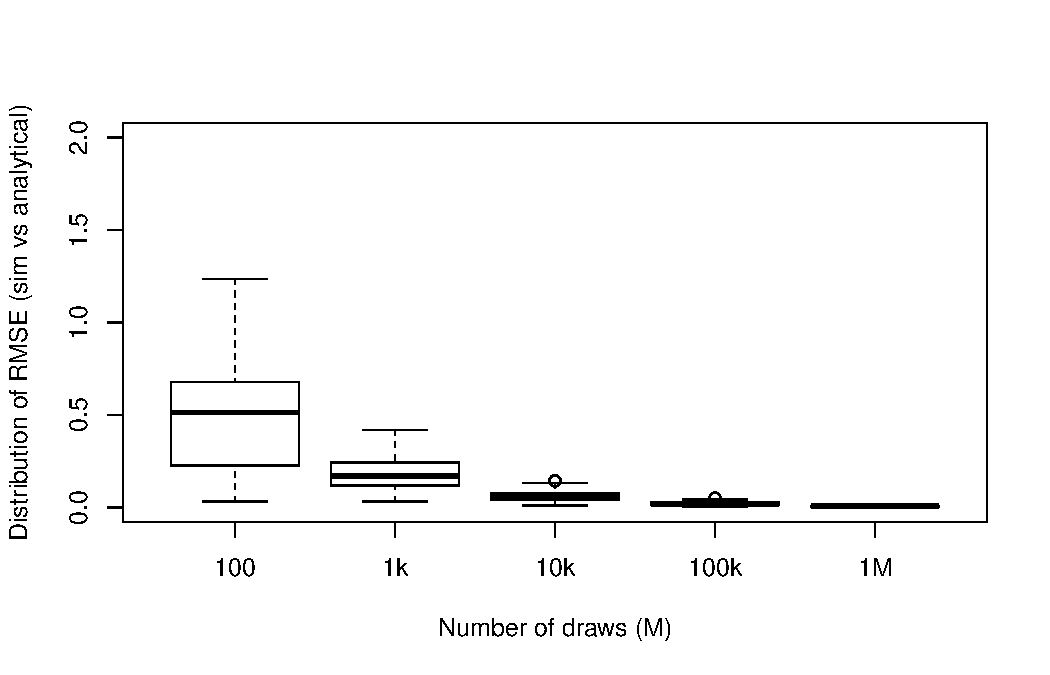
\includegraphics[width=\textwidth]{./../../output/figs/rmses/rmse_boxplots_by_number_of_simulations_no_trunc_dirichlet_v2.pdf}%distribution_of_rmse_across_cases_by_number_of_simulations_test.pdf}
%\end{center} 
%\footnotesize{\text{Note:} For each of 100 sets of belief parameters, we compute pivotal probabilities (1) analytically and (2) by simulation, with $M$ draws from the belief distribution. The figure shows, for each value of $M$ (horizontal axis), the distribution of the average discrepancy (RMSE) between the two approaches across the 100 scenarios.} 
%\end{figure}  

\begin{figure}\caption{Numerical/analytical approach agrees with simulations but is many times faster \label{rmse_box}}
\begin{center}
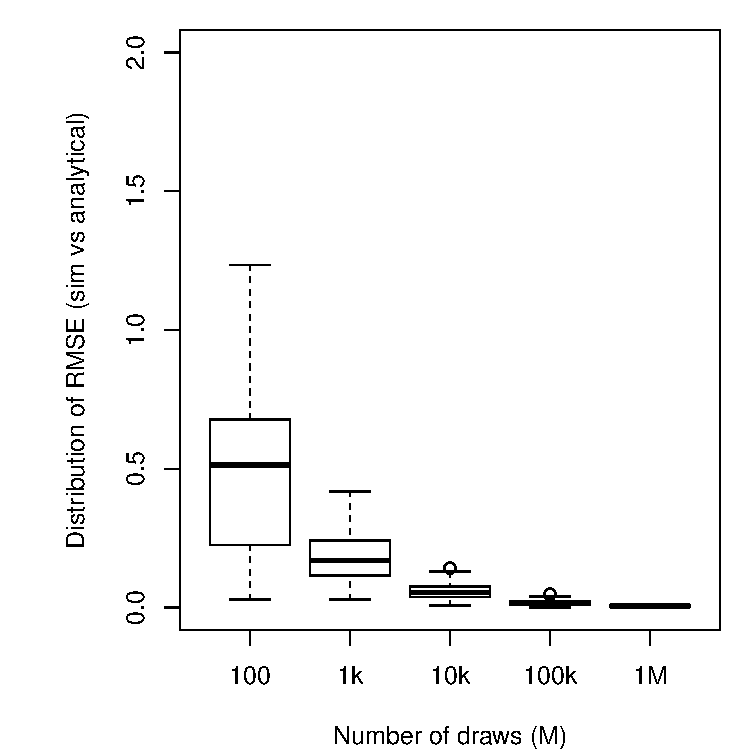
\includegraphics[width=0.5\textwidth]{./../../output/figs/rmses/rmse_boxplots_by_number_of_simulations_no_trunc_dirichlet_v2_narrower.pdf}%distribution_of_rmse_across_cases_by_number_of_simulations_test.pdf}
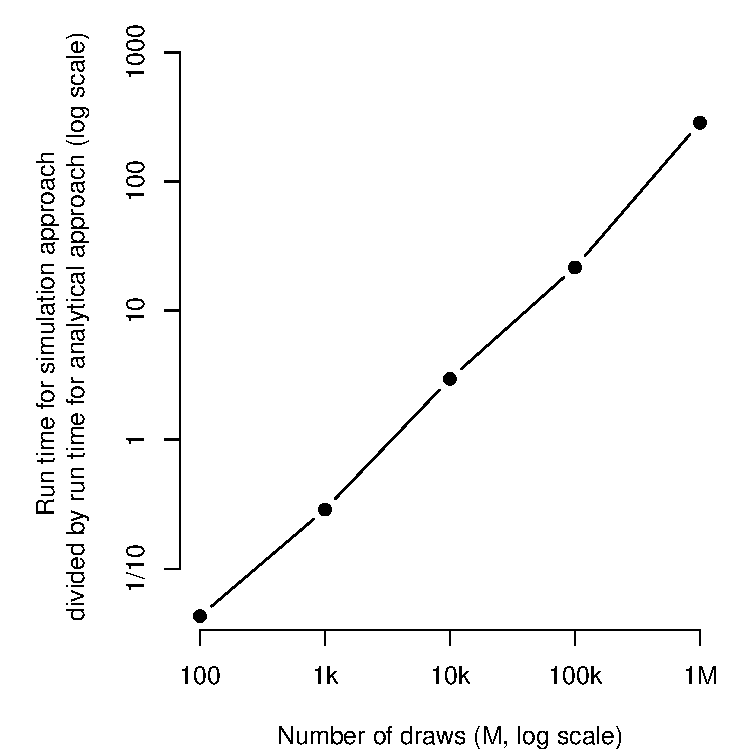
\includegraphics[width=0.5\textwidth]{./../../output/figs/rmses/time_required.pdf}
\end{center} 
\footnotesize{\text{Note:} For each of 100 sets of belief parameters, we compute pivotal probabilities (1) analytically and (2) by simulation, with $M$ draws from the belief distribution. We then calculate the RMSE across the 12 pivotal events between the analytical approach and the simulation approach for each of the 100 scenarios. The left figure shows, for each value of $M$ (horizontal axis), that the distribution of the RMSEs across the 100 scenarios converges to a point mass at zero as the number of simulation draws increases. The right panel shows how the relative computational burden of the simulation approach increases as the number of simulation draws increases} 
\end{figure}  


Second, for each pivotal event we compute at each $M$ the RMSE across the $J=100$ scenarios between $\mathbf{T}$ and $\mathbf{\tilde{T}}_M$. That is, for a given $M$, we compute the RMSE for each column of $\mathbf{T}$ and $\mathbf{\tilde{T}}_M$. Figure \ref{rmse_box} summarizes how these RMSEs vary with $M$. It shows that the RMSE drops toward zero for all pivotal events as the number of number of draws from the belief distribution increases.

\begin{figure}\caption{RMSE by pivotal event and number of draws in simulation \label{rmse_box}}
\begin{center}
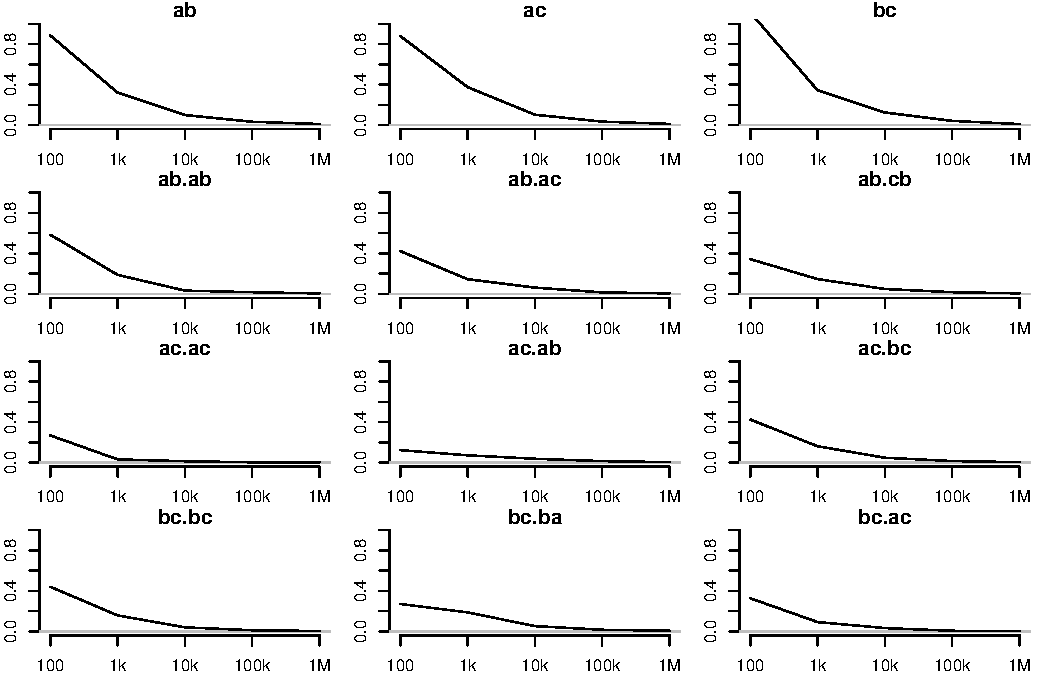
\includegraphics[width=\textwidth]{./../../output/figs/rmses/rmse_by_pivotal_event_by_number_of_simulations_no_trunc_dirichlet_v2.pdf} %rmse_by_pivotal_event_by_number_of_simulations_test.pdf}
\end{center} 
\footnotesize{\text{Note:} For each of 100 sets of belief parameters, we compute pivotal probabilities (1) analytically and (2) by simulation, with $M$ draws from the belief distribution. The figure shows, for each pivotal event, the average discrepancy (RMSE) between the two approaches as $M$ increases.} 
\end{figure}  

% can check the time required 





\end{document} 


